\documentclass[a4paper, 12pt, oneside]{book}
\usepackage[backend=biber, backref=true, sorting=none]{biblatex}
\usepackage{csquotes}
\usepackage{graphicx}
\usepackage{geometry}
\usepackage{setspace}
\usepackage{hyperref}
\usepackage[italian]{babel}
\usepackage{listings}
\usepackage{xcolor}
\usepackage{amsthm}
\usepackage{enumitem}
\usepackage{tikz}
\usepackage{amsmath}
\usepackage{xfrac}
\usepackage{amssymb}
\usepackage{multirow}
\usepackage{array}
\usepackage{makecell}
\usepackage{colortbl}
\usepackage{longtable}
\addbibresource{tesi.bib}

\usepackage{fancyhdr}
\pagestyle{fancy}

\fancyhead[LE,RO]{\slshape\rightmark}
\fancyhead[LO,RE]{\slshape\leftmark}
\fancyfoot[C]{\thepage}

\renewcommand{\chaptermark}[1]{\markboth{\chaptername\ \thechapter:\ #1}{}}
\renewcommand{\sectionmark}[1]{\markright{\thesection\ #1}}

\newcommand{\coloredtextsc}[2]{\textcolor{#1}{\textsc{#2}}}

\newcommand{\qq}[1]{``#1''}

\setquotestyle{italian}

\setlength{\headheight}{14.5pt}

\setlength{\LTpost}{-5pt}

\renewcommand{\contentsname}{Indice}

\newtheoremstyle{normal}
  {\topsep}{\topsep}%
  {\normalfont}{0pt}{\bfseries}{}{5pt}
  {}

\theoremstyle{normal}
\newtheorem{esempio}{Esempio}

\lstset{
  language=Java,
  basicstyle=\small\ttfamily,
  keywordstyle=\color{blue}\bfseries,
  commentstyle=\color{green!60!black}\itshape,
  stringstyle=\color{orange},
  showstringspaces=false,
  breaklines=true,
  numbers=left,
  numberstyle=\tiny,
  frame=single,
  captionpos=b,
  emph={esempio},
  emphstyle=\normalfont,
  mathescape=true
}

\begin{document}

\newgeometry{margin=1in} 
\begin{titlepage}

    \noindent
    \begin{minipage}[t]{0.19\textwidth}
        \vspace{-4mm}{
\includegraphics[scale=1.15]{img/logo.pdf}}
    \end{minipage}
    \begin{minipage}[t]{0.8\textwidth}
    {
        \setstretch{1.42}
        Università degli Studi di Milano Bicocca \\
        \textbf{Scuola di Scienze} \\
        \textbf{Dipartimento di Informatica, Sistemistica e Comunicazione} \\
        \textbf{Corso di laurea in Informatica} \\
        \par
    }
    \end{minipage}

    \noindent
    \vspace{20mm}
    \begin{center}
    {
        \LARGE{
            \textbf{Un classificatore di condizioni non soddisfacibili per migliorare l'efficienza di esecuzione simbolica}
            \par
        }
    }
    \end{center}
    
    \vspace{70mm}

    \noindent
    {\large \textbf{Relatore:} \textit{Prof. Giovanni Denaro}} \\

    \noindent
    {\large \textbf{Co-relatore:} \textit{Prof. Pietro Braione}}
    
    \vspace{15mm}

    \noindent
    \begin{flushright}
        \textbf{\large Relazione della prova finale di:} \\
        \large{\textit{Cristian Piacente}}\\
        \large{\textit{Matricola 866020}}
    \end{flushright}
    
    \vspace{25mm}

    \noindent
    \begin{center}
        {\large{\textbf{Anno Accademico 2022-2023}}}
    \end{center}
    
\end{titlepage}
\restoregeometry

% --- ABSTRACT ---

\newpage
\thispagestyle{plain}
\begin{flushleft}
  \huge{\textbf{Abstract}}
\end{flushleft}
\vspace{1cm}
\textit{In questa trattazione viene discussa la messa a punto di un'euristica da integrare con il progetto TARDIS, generatore automatico di casi di test per programmi Java, per migliorare le prestazioni della tecnica di esecuzione simbolica dinamica applicata in un budget di tempo limitato. Dunque, si ha come obiettivo la generazione di un maggior numero di casi di test, ottimizzando l'uso del tempo a disposizione: ciò viene reso possibile dall'identificazione di condizioni di eseguibilità non soddisfacibili, a cui corrispondono cammini infeasible. L'euristica comprende l'implementazione di un classificatore, basato su machine learning, e un meccanismo che consente di assegnare priorità diverse alle condizioni di eseguibilità, generate durante l'esecuzione simbolica, a seconda del risultato di classificazione: l'idea è quella di farsi guidare dalle condizioni classificate come soddisfacibili. \\ Vengono effettuati degli esperimenti sia su un programma esempio sia su programmi reali più complessi, ottenendo risultati significativi.}

% --- INDICE --- %
\tableofcontents



% --- capitolo 1 - INTRODUZIONE --- %
\chapter{Introduzione}

La costruzione di software di alta qualità richiede attività di verifica (quality assurance) per assicurarsi di rispettare diversi requisiti di qualità, come la robustezza (fault-tolerance): la tecnica di validazione principale consiste nel testing. \\ Il caso ideale sarebbe testare tutti i possibili input (testing esaustivo), ma è impossibile nella pratica poiché gli input tendono a essere infiniti. \\ Per esplorare lo spazio di input di un programma si può ricorrere a tecniche di analisi statica o dinamica. In particolare, l'analisi statica ha l'obiettivo di dedurre proprietà di qualità basandosi sul funzionamento del programma, che risulta finito, mentre con l'analisi dinamica la deduzione si ottiene esaminando tracce di esecuzione del programma. \\ \\ Oggi, una tecnica di analisi statica diffusa è l'esecuzione simbolica: si tratta di associare agli input dei simboli che rappresentano valori arbitrari. In questo ambito di analisi statica, l'esecuzione simbolica tipicamente ha come applicazione la dimostrazione di correttezza di un programma. \\ Invece, un'attuale tecnica di analisi dinamica usata per ottenere un'alta copertura del codice è la cosiddetta esecuzione simbolica dinamica: questa tecnica permette la generazione automatica di casi di test. \\ Nella pratica, la generazione di casi di test avviene sfruttando una tecnica metaeuristica search-based in cui alla fitness function corrisponde la soddisfacibilità delle condizioni di eseguibilità ottenute dall'esecuzione simbolica dinamica. \\ \\ Tuttavia, soprattutto nel caso della programmazione orientata ad oggetti, è necessario identificare sequenze valide di chiamate a metodi per istanziare correttamente gli input non primitivi, rispettando l'interfaccia pubblica che si ha a disposizione. \\ Un generatore automatico di casi di test, che affronta il problema di generare sequenze legali di chiamate a metodi in un contesto di un programma con input complessi, è TARDIS \cite{braione2019sushi}. \\ Dato un programma Java in input, TARDIS combina l'esecuzione simbolica dinamica e la generazione search-based di casi di test per avere in output test JUnit. Un problema rimasto aperto riguarda l'utilizzo ottimale del budget di tempo limitato a disposizione, al fine di massimizzare il numero di casi di test generati, in particolare in uno scenario in cui il programma passato in input presenta un numero elevato di condizioni di eseguibilità non soddisfacibili. \\ \\ In questa trattazione viene presentato un approccio che affronta questo problema: viene definito il funzionamento di un classificatore di condizioni di eseguibilità non soddisfacibili, con lo scopo di non sprecare tempo soffermandosi sulle condizioni non soddisfacibili (poiché portano solo al timeout del generatore di casi di test) e di ottenere una migliore copertura del codice nel budget di tempo prefissato. Dunque, l'euristica permette di classificare le condizioni di eseguibilità alternative, generate dall'esecutore simbolico, come soddisfacibili o non soddisfacibili in base all'esperienza che si ha nel tempo, e di integrare questo meccanismo con il funzionamento di TARDIS tramite un'assegnazione di priorità alle condizioni, a seconda della classificazione prodotta. \\ \\ Questa trattazione è organizzata come segue. Il capitolo \ref{chapter:dse} presenta la tecnica di esecuzione simbolica generalizzata, la tecnica di esecuzione simbolica dinamica (applicata per un esempio particolare) e il funzionamento di TARDIS. Il capitolo \ref{chapter:classifier} tratta elementi introduttivi utilizzati per la messa a punto del classificatore, il funzionamento del classificatore, il meccanismo di assegnazione parametrizzata (usato per assegnare priorità diverse alle condizioni di eseguibilità) e i risultati prodotti per l'esempio particolare visto durante la spiegazione dell'esecuzione simbolica dinamica. Il capitolo \ref{chapter:experiments} descrive gli esperimenti effettuati considerando classi di progetti \qq{reali}, più complesse dell'esempio considerato inizialmente.



% --- capitolo 2 - TEST DSE --- %
\chapter{Test DSE}\label{chapter:dse}

Questo capitolo tratta concetti necessari per comprendere l'obiettivo della ricerca svolta. Lo scopo è quello di presentare la tecnica di esecuzione simbolica dinamica e il funzionamento generale del progetto TARDIS.   
\\ \\ Prima di parlare di esecuzione simbolica dinamica è bene introdurre nozioni sull'esecuzione simbolica generalizzata.

\section{Background: esecuzione simbolica}

\subsection{Nozioni preliminari}

L'esecuzione simbolica \cite{king1976symbolic} generalizzata è una tecnica di analisi statica che consiste nell'eseguire un programma passando come input \textbf{simboli} che rappresentano valori arbitrari, al posto di normali input. \\ L'esecuzione procede come in una normale esecuzione, tranne per il fatto che i valori assunti dalle variabili possono essere formule simboliche che hanno come variabili libere i simboli di input. Di solito lo stato di una normale esecuzione di un programma include i valori delle variabili e un counter che fa riferimento all'istruzione in fase di elaborazione: nell'esecuzione simbolica si tiene traccia anche della \textbf{path condition}, cioè una congiunzione di condizioni simboliche che identificano il cammino considerato e che quindi devono essere rispettate per eseguirlo. \\ Perciò, la tecnica collega il comportamento del programma alla logica, consentendo una rappresentazione della relazione tra gli input del programma e i percorsi di esecuzione all'interno di esso. \\ \\ Un cammino è una sequenza di istruzioni che può essere \textbf{feasible}, se esiste almeno un input concreto $V$ tale che quando il programma viene eseguito con $V$ come input si eseguono le istruzioni lungo il cammino dato, oppure \textbf{infeasible}, se non esiste alcun input concreto che fa eseguire il cammino. \\ \\ Se una path condition è soddisfacibile, una procedura di decisione chiamata \textbf{constraint solver} è in grado di trovare assegnamenti alle variabili libere che soddisfano il vincolo. Tuttavia, l'unica classe di vincoli che oggi può essere risolta in maniera efficiente è quella dei vincoli lineari. \\ \textbf{Z3} \cite{de2008z3} è un esempio di solver automatico efficace che consente di determinare se una formula di logica del primo ordine è soddisfacibile.
\\ \\ Una delle applicazioni della tecnica di esecuzione simbolica generalizzata è la \textbf{dimostrazione formale di correttezza di un programma}: consente di verificare se un programma rispetta la proprietà di correttezza per tutte le possibili esecuzioni senza aver bisogno di eseguire il programma con valori concreti di input, poiché l'esecuzione avviene solo simbolicamente per un insieme di classi di input. \\ Si tratta di una metodologia di testing molto utile perché spesso l'insieme di possibili valori per un dato input è praticamente infinito.

\subsection{Esempio di esecuzione simbolica generalizzata}
Di seguito viene riportato un esempio per comprendere meglio la tipica applicazione della tecnica.
\begin{esempio}
\textit{Tramite la tecnica dell'esecuzione simbolica si vuole stabilire se il seguente programma è corretto o meno rispetto all'oracolo (asserzione alla riga 7)}
\begin{lstlisting}
public static void esempio(int x, int y) {
  if (x > y) {
    x = x + y;
    y = x - y;
    x = x - y;
    assert(x > y);
  }
  System.out.printf("x = %d, y = %d", x, y);
}
\end{lstlisting}
\end{esempio}
\noindent \\ Lo scopo è verificare se è possibile violare l'assert in almeno un cammino. 
\\ Innanzitutto, si può notare che ci sono soltanto 2 possibili cammini: il cammino che segue le istruzioni all'interno del ramo \textit{then}, che possiamo indicare con 2-3-4-5-6-8, e il cammino in cui si esegue il branch \textit{else}, cioè 2-8.
\\ \\ Chiaramente non sarà mai possibile violare l'asserzione nel secondo cammino, in quanto l'istruzione non appartiene al cammino, quindi ci si soffermerà sull'esecuzione del primo.
\\ \\ In base a quanto detto nelle nozioni preliminari, per effettuare un'esecuzione simbolica è indispensabile tener conto dell'\textbf{istruzione corrente}, dei \textbf{valori simbolici} delle variabili e della \textbf{path condition} (come condizioni di eseguibilità si indica true inizialmente).
\\ \\ Come input si considerino i simboli $A$ e $B$, al posto degli input concreti $x$ e $y$.
\\ Per tutti i cammini l'inizializzazione è comune, ossia \verb|dopo la riga 1| si hanno le variabili \verb|x = A, y = B| e come path condition (PC) \verb|true|.
\\ \\ Prendendo in esame il cammino 2-3-4-5-6-8 si ottiene:
\begin{itemize}[label={--}, itemsep=0pt, topsep=2pt]
    \item \verb|dopo 2 (jump to 3):  x = A, y = B,      PC: A > B|
    \item \verb|dopo 3:              x = A + B, y = B,  PC: A > B|
    \item \verb|dopo 4:              x = A + B, y = A,  PC: A > B|
    \item \verb|dopo 5:              x = B, y = A,      PC: A > B|
\end{itemize}
\noindent \\ Ora, per poter violare l'assert dev'essere soddisfacibile la formula \verb|PC && !assert|, dove con \verb|!assert| si intende la condizione simbolica utilizzata all'interno dell'asserzione ma negata, in questo caso alla riga 6 la variabile $x$ contiene il valore simbolico $B$ e la variabile $y$ contiene $A$, dunque come condizione dell'assert negata si ha \verb|!(B > A)|, cioè \lstinline|B $\leq$ A|. \\ Ci si deve chiedere se è soddisfacibile la formula \lstinline|A > B && B $\leq$ A|: la risposta è affermativa e un constraint solver sarebbe in grado di trovare assegnamenti agli input simbolici, ad esempio si può scegliere \verb|A = 1, B = 0| come caso di test che dimostra che l'asserzione non viene sempre soddisfatta. 
\\ \\ Si è dimostrato che \textbf{il programma non risulta corretto rispetto all'oracolo}.

\clearpage

\section{Dynamic Symbolic Execution}\label{section:dse}
Dopo aver trattato l'esecuzione simbolica generalizzata, in questa sezione si parla della sua importante declinazione: l'\textbf{esecuzione simbolica dinamica}.

\subsection{Teoria DSE: funzionamento}
L'esecuzione simbolica dinamica \cite{araki2018systematic, enwiki:1151336533}, conosciuta come Dynamic Symbolic Execution (DSE) oppure concolic execution (CONCrete + symbOLIC), è una tecnica che ha l'obiettivo di \textbf{generare automaticamente casi di test} di un dato programma. Viene eseguita allo stesso tempo concretamente (passando particolari input) e simbolicamente (trattando variabili con valori simbolici), analizzado il comportamento del programma rispetto al suo possibile spazio di input, cioè analizzando cammini diversi rispetto ad assunzioni diverse sugli input. \\ La parte dell'esecuzione simbolica consente di memorizzare i vincoli sugli input simbolici per ogni branch incontrato durante l'esecuzione concreta.
\\ \\ L'idea è quella di \textbf{farsi guidare dai casi di test}, poiché eseguendo un caso di test si segue concretamente un certo cammino del codice: ciò si distingue dalla tecnica di esecuzione simbolica generalizzata perché si evita di scegliere in ordine casuale (o scelto dall'analista) i cammini da analizzare.
\\ \\ Un'altra differenza rispetto all'esecuzione simbolica generalizzata consiste nella sua applicazione. Una delle principali applicazioni ha come obiettivo quello di trovare bug, al posto di dimostrare la proprietà di correttezza del programma. \\ La generazione di casi di test avviene combinando l'esecuzione simbolica con un constraint solver, con lo scopo di massimizzare la copertura del codice. \\ Perciò, la tecnica combina l'analisi simbolica, che porta a generare casi di test, con l'esecuzione dei casi di test, generati per proseguire con l'analisi. 
\\ \\ L'esecuzione simbolica dinamica ha inizio eseguendo il programma con input concreti scelti arbitrariamente (di solito generati randomicamente). \\ L'esecuzione segue un particolare cammino a seconda dei valori di input e viene memorizzata la path condition corrispondente. \\ \\ Nell'esecuzione simbolica generalizzata ci si chiede se una certa path condition è soddisfacibile o non soddisfacibile: nella tecnica DSE questo avviene solo per le path condition ricavate manipolando la formula simbolica, poiché se le condizioni di eseguibilità sono state generate dall'esecuzione di un caso di test si sa per costruzione che esiste un caso di test in grado di eseguire esattamente quel cammino, dunque non è necessario invocare il constraint solver per questi casi. \\ A questo punto l'idea è di esplorare gli altri cammini ma in modo ordinato, cioè utilizzando il caso di test come guida. \\ \\ Vengono generate path condition alternative negando una alla volta le clausole: ciò significa fare assunzioni diverse durante l'esecuzione del test, che permettono di eseguire branch non già coperti. \\ Viene quindi generata una lista di path condition (o prefissi di path condition) alternative prendendo in considerazione tutte le possibili variazioni della path condition considerata. \\ \\ Per ciascuna path condition alternativa \emph{non ridondante} viene invocato il constraint solver (a questo step è necessario) per tentare di generare un caso di test che rispetta le condizioni: se non avviene la risoluzione dei vincoli simbolici allora viene scartata la path condition alternativa, altrimenti si ripete il procedimento sul nuovo input concreto generato a partire dalla path condition alternativa. \\ \\ Dunque, l'idea è di abbandonare il prima possibile i cammini infeasible, a cui corrispondono path condition non soddisfacibili, concentrandosi su quelli feasible e variando le scelte effettuate sui branch durante il cammino per provare a generare nuovi input concreti, che nel complesso permettono di avere in generale un'alta copertura del codice. \\ \\ Tuttavia, in una realtà con un budget di tempo limitato non si può dare per scontato di ottenere sempre un'alta copertura, soprattutto quando si ha un'esplosione di path condition.

\subsection{Pratica DSE: un esempio particolare}
Per assicurarsi di aver compreso il funzionamento e per discutere riguardo a possibili problematiche e limitazioni di questa tecnica, viene riportato un esempio di programma molto particolare.

\clearpage
\begin{esempio}\label{example:mipc}
\textit{Lo scopo è quello di massimizzare il numero di cammini coperti durante l'esecuzione del metodo target}
\begin{lstlisting}
public class MIPC {
  private final int[] a;
  private final int[] b;
  
  public MIPC(int a0, int a1, int a2, int a3, int a4, 
      int b0, int b1, int b2, int b3, int b4, 
      int b5, int b6, int b7, int b8, int b9) {
    a = new int[] {a0, a1, a2, a3, a4};
    b = new int[] {b0, b1, b2, b3, b4, b5, b6, b7, b8, b9};
    for (int elemInB: b) {
      if (elemInB < 0) throw new RuntimeException();
    }
  }
  
  public void setA(int index, int value) {
    this.a[Math.abs(index) % this.a.length] = value;
  }
  
  public boolean target() { /* target method for DSE */
    int k = 0;
    boolean flag = true;
    for (int i = 0; i < a.length; i++) {
      if (a[i] > 1000 + (1000 * i)) {
        for (int j = 0; j < b.length; j++) {
          if (b[j] < -a[i]) { /* infeasible branch */
            k = 1;
          }
        }
      } else {
        flag = false;
      }
    }
    
    if (flag && k == 0) {
      return true;
    } else {
      return false;
    }
  }
}
\end{lstlisting}
\end{esempio}
\subsubsection{Ragionamento preliminare sul codice}
\noindent Innanzitutto, prima di applicare la tecnica DSE è possibile ragionare sulla struttura del codice \ref{example:mipc}, per far emergere alcune osservazioni.
\\ \\ La classe MIPC (ManyInfeasiblePC) ha come attributi due array di interi, inizializzati nel costruttore in cui si nota un \textbf{invariante} da rispettare: l'array \verb|b| non può contenere numeri negativi, altrimenti viene lanciata un'eccezione durante l'istanziazione della classe. \\ Questo significa che per evitare \textbf{falsi positivi} non è sufficiente controllare con un constraint solver che dal punto di vista della logica una certa path condition alternativa sia soddisfacibile, ma si dovrà anche tener conto delle \textbf{precondizioni} del programma che si sta testando, poiché in questo caso l'esecuzione di un caso di test violerebbe le assunzioni: si tratta di una \emph{limitazione} della tecnica di esecuzione simbolica dinamica.
\\ Si ha poi un metodo setter, che si può ignorare per il momento, seguito dalla parte più importante della classe: il metodo target, considerato durante l'applicazione della tecnica.
\\ Per ogni elemento dell'array \verb|a|, di lunghezza 5, vi sono due branch, entrambi feasible in quanto l'array \verb|a| non ha alcuna limitazione. \\ Tuttavia, se viene eseguito il ramo \textit{then}, vi è un altro ciclo innestato: per ogni elemento dell'array \verb|b|, di lunghezza 10, c'è un branch \textbf{infeasible}. \\ In tutto, \textbf{il numero di cammini feasible è $2^{\;a.length} = 2^5 = 32$}, mentre ci sono centinaia di path condition non soddisfacibili a cui corrispondono cammini infeasible: da qui il nome della classe. \\ Nella realtà, avendo a disposizione un budget di tempo limitato è necessario definire un'\textbf{euristica} che permette di guidare la tecnica discriminando le path condition a cui corrispondono cammini feasible: un \textbf{approccio per migliorare l'efficienza} dell'esecuzione simbolica dinamica viene trattato nel capitolo \ref{chapter:classifier}.
\subsubsection{Applicazione tecnica DSE}
Viene descritto un esempio di esecuzione simbolica dinamica.
\paragraph{Input concreto arbitrario} Il programma viene eseguito con un caso di test scelto arbitrariamente, poiché non vi è ancora una path condition da rispettare (si potrebbe considerare come \verb|true|, per fare un'analogia con l'esecuzione simbolica generalizzata). Supponendo che la classe venga inizializzata passando al costruttore il valore $0$ ripetuto 5 volte per l'array \verb|a| e 10 volte per l'array \verb|b|, risulta:
\begin{lstlisting}[numbers=none, frame=none, basicstyle=\fontsize{10}{12}\selectfont\ttfamily]
MIPC mipc = new MIPC(0, 0, 0, 0, 0, 0, 0, 0, 0, 0, 0, 0, 0, 0, 0);
boolean targetRes = mipc.target();
\end{lstlisting}
\paragraph{Path condition e generazione path condition alternative} Durante l'esecuzione del programma vengono calcolate le condizioni di eseguibilità e in seguito si generano le path condition alternative. 
\\ Indicando con i simboli $A$ e $B$ gli array \verb|this.a| e \verb|this.b|, si ha come path condition: \begin{lstlisting}[numbers=none, frame=none, basicstyle=\fontsize{10}{12}\selectfont\ttfamily]
A.length $\geq$ 0 && 0 < A.length && A[0] $\leq$ 1000 && 1 < A.length && 
 A[1] $\leq$ 2000 && 2 < A.length && A[2] $\leq$ 3000 && 3 < A.length && 
 A[3] $\leq$ 4000 && 4 < A.length && A[4] $\leq$ 5000 && 5 $\geq$ A.length
\end{lstlisting}
Questo perché innanzitutto concretamente l'array \verb|this.a| non è \verb|null| bensì un nuovo oggetto nello heap (da qui la prima clausola simbolica), poi si entra nel ciclo più esterno 5 volte e viene sempre eseguito il branch \verb|else| alla riga 29, dunque si nega la condizione dell'if alla riga 23. L'ultima clausola corrisponde alla condizione di uscita del ciclo, cioè la negazione di \verb|5 < A.length|.
\\ A questo punto, è bene fare un accorgimento prima di generare le path condition alternative: per gli input di tipo reference è necessario tenere in considerazione diverse possibili \textbf{assunzioni}. Infatti, è possibile avere uno dei tre seguenti scenari:
\begin{enumerate}[itemsep=0pt, topsep=2pt]
    \item il reference in input è \verb|null|
    \item il reference in input è un \verb|alias| di un altro input
    \item il reference in input è un \verb|nuovo oggetto| nello heap
\end{enumerate}
Il punto 3 è quello che si è ottenuto con il caso di test iniziale, il punto 2 si considera solo quando vengono coinvolti almeno due input (nella path condition si può notare che non vi è alcuna condizione che dipende dall'array \verb|b|), mentre il punto 1 si può usare per generare la prima path condition alternativa.
\\ Considerando quanto appena detto e negando una alla volta le clausole, si ottiene la seguente lista di path condition alternative:
\begin{itemize}[itemsep=0pt, topsep=2pt]
    \item \lstinline|A == null|
    \item \lstinline|A.length $\geq$ 0 && 0 $\geq$ A.length|
    \item \lstinline|A.length $\geq$ 0 && 0 < A.length && A[0] > 1000|
    \item \lstinline|A.length $\geq$ 0 && 0 < A.length && A[0] $\leq$ 1000 && 1 $\geq$ A.length|
    \item \lstinline|A.length $\geq$ 0 && 0 < A.length && A[0] $\leq$ 1000 && 1 < A.length| \\
\lstinline|&& A[1] > 2000|
    \item \lstinline|A.length $\geq$ 0 && 0 < A.length && A[0] $\leq$ 1000 && 1 < A.length| \\
\lstinline|&& A[1] $\leq$ 2000 && 2 $\geq$ A.length|
    \item \lstinline|A.length $\geq$ 0 && 0 < A.length && A[0] $\leq$ 1000 && 1 < A.length| \\
\lstinline|&& A[1] $\leq$ 2000 && 2 < A.length && A[2] > 3000|
    \item \lstinline|A.length $\geq$ 0 && 0 < A.length && A[0] $\leq$ 1000 && 1 < A.length| \\
\lstinline|&& A[1] $\leq$ 2000 && 2 < A.length && A[2] $\leq$ 3000 && 3 $\geq$ A.length|
    \item \lstinline|A.length $\geq$ 0 && 0 < A.length && A[0] $\leq$ 1000 && 1 < A.length| \\
\lstinline|&& A[1] $\leq$ 2000 && 2 < A.length && A[2] $\leq$ 3000 && 3 < A.length| \\
\lstinline|&& A[3] > 4000|
    \item \lstinline|A.length $\geq$ 0 && 0 < A.length && A[0] $\leq$ 1000 && 1 < A.length| \\
\lstinline|&& A[1] $\leq$ 2000 && 2 < A.length && A[2] $\leq$ 3000 && 3 < A.length| \\
\lstinline|&& A[3] $\leq$ 4000 && 4 $\geq$ A.length|
    \item \lstinline|A.length $\geq$ 0 && 0 < A.length && A[0] $\leq$ 1000 && 1 < A.length| \\
\lstinline|&& A[1] $\leq$ 2000 && 2 < A.length && A[2] $\leq$ 3000 && 3 < A.length| \\
\lstinline|&& A[3] $\leq$ 4000 && 4 < A.length && A[4] > 5000|
    \item \lstinline|A.length $\geq$ 0 && 0 < A.length && A[0] $\leq$ 1000 && 1 < A.length| \\
\lstinline|&& A[1] $\leq$ 2000 && 2 < A.length && A[2] $\leq$ 3000 && 3 < A.length| \\
\lstinline|&& A[3] $\leq$ 4000 && 4 < A.length && A[4] $\leq$ 5000 && 5 < A.length| \\
\end{itemize}
Si può fare una considerazione: col progredire dell'esecuzione, durante la generazione delle path condition alternative si possono riscontrare vincoli ridondanti (già coperti da un caso di test) che è meglio scartare a priori.
\paragraph{Risoluzione vincoli e generazione nuovo input concreto} Dopo aver escluso eventuali path condition ridondanti, si può invocare un constraint solver per eliminare le condizioni di eseguibilità composte da clausole che si contraddicono. \\ Per questo esempio non è possibile generare casi di test usando direttamente il solver, perché non si hanno costanti numeriche come input ma \textbf{reference}: si deve ricorrere a un \textbf{tool di generazione automatica di casi di test}, come \textbf{EvoSuite} \cite{fraser2011evosuite}. Questa è un'altra limitazione della tecnica DSE. \\ Ora, si seleziona una path condition da passare al generatore di casi di test, con lo scopo di ottenere input concreti a cui corrispondono le condizioni simboliche. Nella realtà si tratta di uno step delicato, in quanto se si sceglie una path condition non soddisfacibile allora il tool andrà in \textbf{timeout} e viene sprecato del tempo. Supponendo di avere a disposizione un'euristica in grado di \textbf{classificare} le nuove path condition come non soddisfacibili o soddisfacibili, \textit{e supponendo di non avere un training set vuoto all'inizio}, cominciando dall'alto in questo esempio viene selezionata la terza path condition, a cui corrisponde un cammino feasible perché rispetta l'invariante della lunghezza dell'array \verb|a|. Invece, senza alcuna euristica viene selezionata la prima path condition, che è certamente non soddisfacibile e dunque il tool di generazione di casi di test andrà in timeout: l'ordine di esplorazione delle path condition ha un importante impatto sull'\textbf{efficienza} ed è quello di cui si occupa l'attività svolta. \\ A questo punto, una volta selezionata una path condition soddisfacibile è stato generato un nuovo input concreto: si replica quanto svolto, a partire dall'esecuzione del programma col nuovo caso di test per ottenere nuove condizioni di soddisfacibilità da considerare. \\ La tecnica si interrompe nel momento in cui non vi è più alcuna path condition soddisfacibile non ridondante tra quelle alternative (oppure quando si esaurisce il budget di tempo a disposizione).

\section{TARDIS: schema di funzionamento}
Questa sezione ha lo scopo di mostrare una panoramica riguardo alla struttura generale del progetto utilizzato durante l'esperienza, in modo da poter capire meglio su quale parte concentrarsi. 
\\ \\ TARDIS \cite{braione2019sushi} (me\textbf{TA}heu\textbf{R}istically-driven \textbf{D}ynam\textbf{I}c \textbf{S}ymbolic execution) è un generatore automatico di casi di test per programmi Java e ha l'obiettivo di ottenere un'alta copertura dei branch. \\ È in grado di gestire sia programmi con input primitivi sia quelli con input complessi (strutture dati) \cite{braione2017combining}. \\ \\ Viene sfruttata l'esecuzione simbolica per analizzare i cammini del programma e generare path condition, focalizzando l'attenzione sui cammini che portano a branch non ancora coperti. Queste path condition vengono passate a una versione modificata di EvoSuite, che utilizza una tecnica metaeuristica search-based (in particolare un algoritmo genetico \cite{enwiki:1158719624}) per produrre in output casi di test JUnit che eseguono i cammini. \\ In particolare, viene alternata l'esecuzione simbolica svolta dall'esecutore simbolico \textbf{JBSE} (Java Bytecode Symbolic Executor) \cite{braione2016jbse} con la generazione di casi di test di cui si occupa \textbf{EvoSuite}. \\ \\ Perciò, TARDIS combina la tecnica DSE, trattata nella sezione \ref{section:dse}, con la generazione search-based di casi di test: lo scopo è quello di trarre vantaggio dall'esecuzione simbolica calcolando le condizioni di eseguibilità di branch difficili da coprire e dalla capacità dei generatori search-based di casi di test di costruire input concreti complessi tramite una sequenza \emph{legale} di invocazioni a costruttori e modificatori (motivo per cui alla riga 15 dell'esempio \ref{example:mipc} vi è un metodo setter per l'array A, altrimenti EvoSuite fa molta più fatica a generare un caso di test), assicurando di non avere falsi positivi poiché si utilizza l'API disponibile del programma che si sta testando.
\clearpage
\begin{figure}[h]
  \centering
  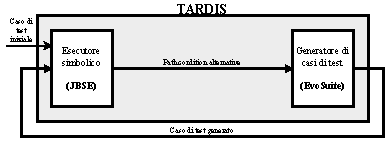
\includegraphics[width=\textwidth]{img/tardis-diagram.pdf}
  \caption{Schema di funzionamento di TARDIS}
  \label{diagram:tardis-workflow-no-classifier}
\end{figure}
\noindent Analogamente all'esecuzione simbolica dinamica, TARDIS inizia la propria esecuzione considerando un caso di test iniziale, che può essere generato randomicamente oppure passato come input da riga di comando (di solito viene utilizzata la prima opzione), poi viene eseguito JBSE per calcolare la path condition corrispondente al cammino seguito durante l'esecuzione del caso di test. \\ A questo punto TARDIS genera una lista di path condition alternative, negando le condizioni dei branch attraversati, e le passa al modulo che si occupa della generazione di test, cioè vengono date in input ad EvoSuite utilizzando come fitness function la soddisfacibilità delle formule simboliche. \\ TARDIS termina l'esecuzione quando non ci sono altre path condition da analizzare oppure quando scade il budget di tempo globale. \\ \\ Uno svantaggio di questo tool è che sia l'esecuzione simbolica sia la generazione di casi di test sono processi costosi dal punto di vista computazionale.
\\ \\ La novità, presentata nel capitolo \ref{chapter:classifier}, consiste in un \textbf{classificatore} che permette a TARDIS di dare una priorità alle path condition alternative soddisfacibili, rispetto a quelle non soddisfacibili, in modo tale che nel momento in cui si scelgono le path condition da passare ad EvoSuite si ha un criterio che non fa sprecare tempo.


% --- capitolo 3 - APPROCCIO: CLASSIFICATORE --- %
\chapter{Approccio: classificatore}\label{chapter:classifier}

In questo capitolo lo scopo principale è la trattazione dell'euristica che consente la classificazione di nuove path condition, cioè l'approccio utilizzato per migliorare l'efficienza della tecnica DSE, trattata nel capitolo \ref{chapter:dse}, facendo riferimento all'esempio \ref{example:mipc} per far fronte al problema dell'esplosione di path condition non soddisfacibili. \\ \\ Inizialmente vengono discussi alcuni concetti fondamentali, e la terminologia, per lo sviluppo del classificatore, in seguito viene presentato il funzionamento del classificatore, il meccanismo di assegnazione \emph{parametrizzata} di una path condition ad una coda (e la relativa estrazione probabilistica) e infine i risultati prodotti effettuando esecuzioni, di diverso tipo, dell'esempio MIPC.

\section{Elementi introduttivi}

\subsection{Slicing, contesto e infeasibility core}

Lo \textbf{slicing} di una path condition è una procedura che consente di dividere una path condition in due sottoformule indipendenti. \\ Due formule simboliche sono dipendenti se e solo se esiste almeno una variabile condivisa da entrambe. \\ Quello che viene tenuto in considerazione è la \textbf{chiusura transitiva della relazione di dipendenza} tra formule, in particolare si calcolano tutte le condizioni dipendenti, direttamente o indirettamente, dall'\textbf{ultima clausola}. \\ Il motivo per cui si effettua la chiusura transitiva della relazione di dipendenza dall'ultima clausola consiste nella seguente osservazione: tenendo conto di una path condition alternativa ottenuta negando l'ultima clausola di una path condition, se essa risulta non soddisfacibile allora è sicuramente dovuto all'ultima clausola, ma non è detto che sia l'unica clausola a rendere tutta la formula una contraddizione. \\ Infatti, potrebbero esserci altre clausole che messe in AND con l'ultima clausola rendono il tutto non soddisfacibile. \\ \\ Perciò, una delle due sottoformule indipendenti si ottiene nel seguente modo: si considera l'ultima clausola della path condition alternativa che certamente appartiene a questa sottoformula, poi per ogni altra clausola si controlla \emph{transitivamente} se questa è dipendente dalla sottoformula corrente, se è così allora la condizione simbolica viene aggiunta alla sottoformula. \\ Il risultato di questa operazione è chiamato \textbf{infeasibility core}: è una sottoformula ottenuta dalla chiusura transitiva della relazione di dipendenza a partire dalla sottoformula contenente solo l'ultima clausola della path condition alternativa. \\ \\ Tutte le altre clausole, non appartenenti all'infeasibility core, costituiscono una sottoformula indipendente chiamata \textbf{contesto}: per costruzione è sempre \textbf{soddisfacibile}, poiché si ottiene indipendentemente dall'infeasibility core a partire da una path condition soddisfacibile a cui corrisponde il cammino eseguito da un caso di test concreto. Ciò significa che l'unione tra infeasibility core e contesto restituisce tutta la path condition alternativa, mentre l'intersezione è vuota (essendo due sottoformule indipendenti). \\ \\ Di seguito viene riportato un esempio per chiarire il concetto. \\
\begin{esempio}
\textit{Si considerino le seguenti formule e si applichi la procedura di slicing alla path condition alternativa:} \\ \\
\coloredtextsc{blue}{Path condition} \\
\lstinline|A.length $\geq$ 0 && 0 < A.length && A[0] > 1000 && B.length $\geq$ 0| \\
\lstinline|&& 0 < B.length && B[0] $\geq$ -A[0] && 1 < B.length && B[1] $\geq$ -A[0]| \\
\lstinline|&& 2 < B.length && B[2] $\geq$ -A[0] && 3 < B.length && B[3] $\geq$ -A[0]| \\
\lstinline|&& 4 < B.length && B[4] $\geq$ -A[0] && 5 < B.length && B[5] $\geq$ -A[0]| \\ \lstinline|&& 6 < B.length && B[6] $\geq$ -A[0] && 7 < B.length && B[7] $\geq$ -A[0]| \\ \lstinline|&& 8 < B.length && B[8] $\geq$ -A[0] && 9 < B.length && B[9] $\geq$ -A[0]| \\ \lstinline|&& 10 $\geq$ B.length && 1 < A.length && A[1] $\leq$ 2000 && 2 < A.length| \\ \lstinline|&& A[2] $\leq$ 3000 && 3 < A.length && A[3] $\leq$ 4000 && 4 < A.length| \\ \lstinline|&& A[4] > 5000 && B[0] $\geq$ -A[4] && B[1] $\geq$ -A[4]| \\ \\
\coloredtextsc{blue}{Path condition alternativa, abbreviata per questioni di leggibilità} \\
\lstinline|$\ldots$ && B[1] < -A[4]|
\end{esempio}
\clearpage \noindent Innanzitutto si considerano le variabili (simboliche, a cui si associa un valore arbitrario) dell'ultima clausola della path condition alternativa. \\ 
Le variabili in questione sono \verb|B[1]| e \verb|A[4]|. \\ Ciò significa che per adesso l'infeasibility core risulta \underline{\lstinline|B[1] < -A[4]|}. \\ In seguito si controllano tutte le altre clausole \textbf{in maniera transitiva}. \\ Da una prima iterazione emergono le seguenti clausole che formano una sottoformula dipendente dalla sottoformula contenente solo l'ultima clausola:
\begin{itemize}[itemsep=0pt, topsep=2pt]
    \item \lstinline|B[0] $\geq$ -A[4]|
    \item \lstinline|A[4] > 5000|
    \item \lstinline|B[1] $\geq$ -A[0]|
    \item \lstinline|B[0] $\geq$ -A[0]|
    \item \lstinline|A[0] > 1000|
\end{itemize}
\noindent \\ Ora occorre considerare anche le nuove variabili \verb|B[0]| e \verb|A[0]|, in quanto transitivamente permettono di ottenere una dipendenza. Si effettua un'altra iterazione, considerando le clausole scartate nella precedente iterazione, e si ripete il procedimento finché non vengono più trovate nuove clausole da includere nell'infeasibility core. Dalla seconda iterazione si trovano le seguenti nuove clausole:
\begin{itemize}[itemsep=0pt, topsep=2pt]
    \item \lstinline|B[9] $\geq$ -A[0]|
    \item \lstinline|B[8] $\geq$ -A[0]|
    \item \lstinline|B[7] $\geq$ -A[0]|
    \item \lstinline|B[6] $\geq$ -A[0]|
    \item \lstinline|B[5] $\geq$ -A[0]|
    \item \lstinline|B[4] $\geq$ -A[0]|
    \item \lstinline|B[3] $\geq$ -A[0]|
    \item \lstinline|B[2] $\geq$ -A[0]|
\end{itemize}
\noindent \\ Tenendo in considerazione anche le nuove variabili \verb|B[9]|, \verb|B[8]|, \verb|B[7]|, \verb|B[6]|, \verb|B[5]|, \verb|B[4]|, \verb|B[3]|, \verb|B[2]| non vengono trovate nuove clausole e si interrompe il ciclo.
\noindent \\ \\ In tutto, ordinatamente, l'\textbf{infeasibility core} risulta: \\
\lstinline|A[0] > 1000 && B[0] $\geq$ -A[0] && B[1] $\geq$ -A[0] && B[2] $\geq$ -A[0]| \\
\lstinline|&& B[3] $\geq$ -A[0] && B[4] $\geq$ -A[0] && B[5] $\geq$ -A[0] && B[6] $\geq$ -A[0]| \\
\lstinline|&& B[7] $\geq$ -A[0] && B[8] $\geq$ -A[0] && B[9] $\geq$ -A[0] && A[4] > 5000| \\
\lstinline|&& B[0] $\geq$ -A[4] &&| \underline{\lstinline|B[1] < -A[4]|}
\clearpage \noindent Di conseguenza, il \textbf{contesto}, ottenuto dalla differenza tra l'insieme delle clausole della path condition alternativa e l'insieme di quelle dell'infeasibility core, che si ottiene è: \\
\lstinline|A.length $\geq$ 0 && 0 < A.length && B.length $\geq$ 0 && 0 < B.length| \\
\lstinline|&& 1 < B.length && 2 < B.length && 3 < B.length && 4 < B.length| \\
\lstinline|&& 5 < B.length && 6 < B.length && 7 < B.length && 8 < B.length| \\
\lstinline|&& 9 < B.length && 10 $\geq$ B.length && 1 < A.length && A[1] $\leq$ 2000| \\ \lstinline|&& 2 < A.length && A[2] $\leq$ 3000 && 3 < A.length && A[3] $\leq$ 4000| \\
\lstinline|&& 4 < A.length|

\subsection{Abstraction (terminologia)}

Con il termine abstraction si tende l'eliminazione delle costanti numeriche da una path condition \qq{concreta}, ottenendo in output una path condition \qq{astratta}. \\ \\ Il concetto di abstraction è importante perché è utilizzato nella procedura di slicing per ottenere, oltre all'infeasibility core concreto e al contesto concreto, sia l'\textbf{infeasibility core astratto} sia il \textbf{contesto astratto} di una path condition: essi risultano necessari per l'implementazione dell'euristica.

\subsection{Bloom Filter}

Un \textbf{Bloom Filter} \cite{enwiki:1158711110} è una struttura dati probabilistica efficiente in termini di spazio, utilizzata per controllare se un elemento appartiene a un insieme. \\ Sono possibili falsi positivi, ma \textbf{non sono possibili falsi negativi}. \\ \\ L'idea è quella di mappare elementi, appartenenti a un insieme, a valori tramite diverse funzioni di hash. \\ \\ Un Bloom Filter vuoto è un array di $m$ bit settati a 0. Si hanno $k$ diverse funzioni di hash che mappano un elemento a una delle $m$ posizioni dell'array. \\ \\ Per aggiungere un elemento al Bloom Filter si passa l'elemento a ciascuna delle $k$ funzioni di hash e si settano i bit a 1 nelle posizioni calcolate. \\ \\ Per controllare se un elemento appartiene all'insieme di elementi mappati nel Bloom Filter, si calcolano $k$ posizioni nell'array tramite le funzioni di hash: se vi è un bit settato a 0 in almeno una di queste posizioni allora l'\textbf{elemento definitivamente non appartiene all'insieme} (motivo per cui non si possono riscontrare falsi negativi in questa struttura dati), altrimenti se tutti i bit sono settati a 1 risulta che l'elemento \emph{potrebbe} appartenere all'insieme (quindi si possono avere falsi positivi, se i bit sono stati settati a 1 durante l'aggiunta di altri elementi). \\ Si possono avere situazioni in cui una posizione dell'array è stata settata a 1 dall'hashing di più di un elemento: questo comporta che non è possibile eliminare un elemento dal Bloom Filter, altrimenti si introduce il rischio di avere falsi negativi. \\ \\ Dato un elemento, le operazioni che permettono di aggiungerlo al Bloom Filter e di controllare se esso appartiene all'insieme avvengono in \textbf{tempo costante} $\mathcal{O}(1)$: si tratta dell'unica struttura dati con spazio costante che consente di avere questa caratteristica.
\\ \\ Di seguito è riportato un esempio di Bloom Filter usato per rappresentare l'insieme $\{x, y, z\}$. Vengono utilizzate $k = 3$ funzioni di hash e l'array contiene in tutto $m = 18$ bit. Si ha che l'elemento $w$ non appartiene all'insieme perché l'ultimo bit è settato a 0. \\
\begin{figure}[h]
  \centering
  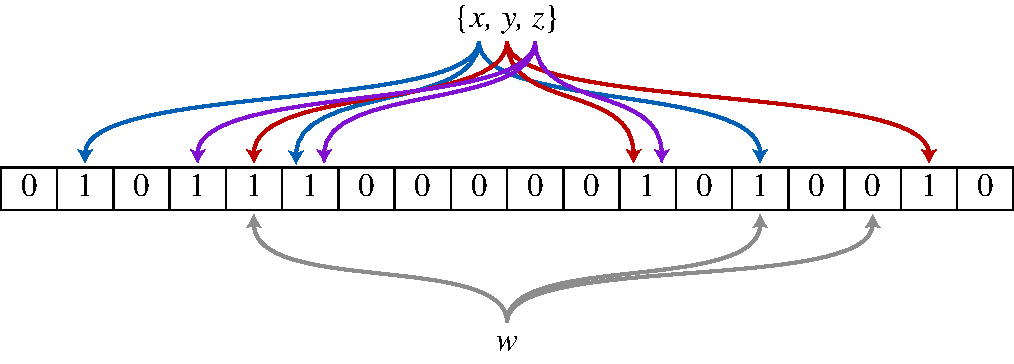
\includegraphics[width=\textwidth]{img/Bloom_filter.pdf}
  \caption{Esempio di Bloom Filter \cite{svgbloomfilter}}
\end{figure}

\subsection{Coefficiente di similarità di Jaccard}

L'\textbf{indice Jaccard} \cite{enwiki:1156109434}, conosciuto anche come coefficiente di similarità di Jaccard, è una statistica utilizzata per misurare la similarità tra insiemi di cardinalità finita. Il coefficiente Jaccard è definito dal rapporto tra la cardinalità dell'intersezione e la cardinalità dell'unione di due insiemi: \[
J(A,B) = {{|A \cap B|}\over{|A \cup B|}} = {{|A \cap B|}\over{|A| + |B| - |A \cap B|}}
\] \clearpage \noindent Si ha che $J(A,B) \in [0, 1]$ e inoltre è possibile calcolare la dissimilarità (\emph{distanza Jaccard}) come il complementare dell'indice Jaccard, ossia $d_J(A,B) = 1 - J(A,B)$.
\\ \\ Per l'implementazione dell'euristica, il coefficiente di similarità di Jaccard viene calcolato tra due \emph{Bloom Filter}, in particolare tra i \textbf{contesti} di due path condition. \\ \\ Dati due Bloom Filter $A$ e $B$, entrambi di lunghezza $n$, si considerino le seguenti definizioni:
\begin{itemize}[label={}, itemsep=0pt, topsep=2pt]
    \item $M_{11}$ indica il numero di posizioni in cui sia $A$ sia $B$ hanno il bit settato a 1
    \item $M_{01}$ indica il numero di posizioni in cui $A$ ha il bit settato a 0 mentre $B$ a 1
    \item $M_{10}$ indica il numero di posizioni in cui $A$ ha il bit settato a 1 mentre $B$ a 0
    \item $M_{00}$ indica il numero di posizioni in cui sia $A$ sia $B$ hanno il bit settato a 0
\end{itemize}
\noindent \\ In tutto si ha $M_{11} + M_{01} + M_{10} + M_{00} = n$ e il \textbf{coefficiente di similarità di Jaccard}, calcolato tra i due Bloom Filter $A$ e $B$, è dato da \[
J = {M_{11} \over M_{01} + M_{10} + M_{11}}
\] \\
Perciò, il coefficiente di similarità di Jaccard corrisponde al rapporto tra il numero di bit settati a 1 in entrambi i Bloom Filter e il numero di bit settati a 1 in \emph{almeno} uno dei due Bloom Filter (ossia il bit non è settato a 0 in entrambi i Bloom Filter).

\clearpage
\section{Euristica}
In questa sezione vengono trattati il funzionamento e l'integrazione di un'euristica che permette di classificare le path condition alternative come soddisfacibili o non soddisfacibili, con lo scopo di dare maggior priorità alle prime.

\subsection{Nuovo schema di funzionamento di TARDIS}
L'euristica consiste nell'utilizzo di un classificatore basato sull'algoritmo \textbf{KNN} (K-Nearest Neighbors) con il parametro $K = 1$, cioè l'appartenenza di una nuova path condition alla classe delle path condition soddisfacibili o a quella delle path condition non soddisfacibili dipende dalla path condition più \qq{vicina} nel training set.
\\ \\ Prima di parlare del classificatore è bene mostrare il nuovo schema di funzionamento di TARDIS con l'aggiunta del classificatore: 
\begin{figure}[h]
  \centering
  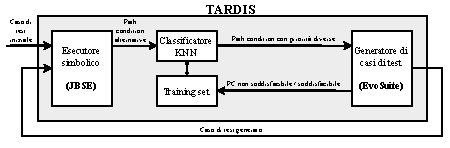
\includegraphics[width=\textwidth]{img/tardis-diagram-classifier.pdf}
  \caption{Nuovo schema di funzionamento di TARDIS}
  \label{diagram:tardis-workflow-classifier}
\end{figure}
\\ Il classificatore prende in input una nuova path condition alternativa, la confronta con il training set per classificarla e viene utilizzato un meccanismo basato su code di priorità diverse per assegnarla a una coda. Tramite un'estrazione probabilistica si sceglie la coda da cui estrarre una path condition e passarla al generatore di casi di test. Se EvoSuite riesce a generare un caso di test che rispetta la path condition allora essa viene inserita nel training set come soddisfacibile, altrimenti se la generazione fallisce si ha che viene messa nel training set come non soddisfacibile. Perciò, il training set aumenta la sua dimensione durante l'esecuzione di TARDIS.

\clearpage
\subsection{Classificatore}
Di seguito viene discusso il funzionamento del classificatore senza fare riferimento a dettagli implementativi di Java.
\subsubsection{Premesse}
Innanzitutto è necessario fare alcune premesse. \\ Ad ogni path condition è associata una struttura dati composta da:
\begin{itemize}[label=$\bullet$, itemsep=0pt, topsep=2pt]
    \item un \verb|Bloom Filter| che rappresenta tutte le clausole del \textbf{contesto}, sia \textbf{concrete} sia \textbf{astratte} (ottenute con l'abstraction), di lunghezza 64 bit. \\ Se non vi è alcuna clausola nel contesto allora il Bloom Filter non contiene alcun bit settato a 1. \\ Questo attributo viene indicato con \verb|context|
    \item un \verb|Bloom Filter| che rappresenta tutte le clausole dell'\textbf{infeasibility core concreto}, di lunghezza 128 bit. \\ Questo attributo viene indicato con \verb|specificInfeasibilityCore|
    \item un \verb|Bloom Filter| che rappresenta tutte le clausole dell'\textbf{infeasibility core astratto}, di lunghezza 128 bit. \\ Questo attributo viene indicato con \verb|generalInfeasibilityCore|
    \item una \verb|lista di oggetti| in cui ciascuno rappresenta \textbf{una clausola} \linebreak dell'\textbf{infeasibility core}, memorizzando distintamente la clausola \textbf{concreta} e quella \textbf{astratta} tramite l'utilizzo di \textbf{due Bloom Filter}: in altre parole vengono sfruttati gli ultimi due attributi considerando come infeasibility core solo una clausola, mentre il Bloom Filter \verb|context| non contiene alcun elemento. \\ Questo attributo viene indicato con \verb|coreBloomFilters|
\end{itemize}
\begin{figure}[h]
  \centering
  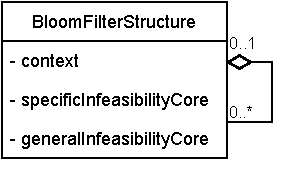
\includegraphics{img/bloom-filter-structure-diagram.pdf}
  \caption{Diagramma delle classi che rappresenta la struttura Bloom Filter}
  \label{diagram:bloom-filter-structure}
\end{figure}
Vengono utilizzate 3 funzioni di hash per mappare ciascuna clausola.
\\ Poiché a una path condition $p$ corrisponde una sola istanza di questa struttura, con abuso di notazione usando \lstinline|$p$.attributo| ci si riferisce a un attributo della struttura associata alla path condition $p$. \\ Un altro abuso di notazione è il seguente: con \qq{item feasible} si intende una path condition soddisfacibile nel training set, così come con \qq{item infeasible} viene indicata una path condition non soddisfacibile nel training set.

\subsubsection{Similarità e funzionamento}
A questo punto è possibile descrivere il funzionamento del classificatore.
\\ In primo luogo, si deve stabilire come calcolare la \textbf{similarità} tra due path condition, poiché in un classificatore KNN è fondamentale definire il concetto di distanza (il complementare della similarità) per poter effettuare la classificazione. \\ \\ La similarità tra due path condition $p_1$ e $p_2$ viene indicata da una \textbf{coppia} $\langle x, y \rangle$, con $x \in [0, 1]$ e $y \in [0, 1]$, in cui $y$ indica il coefficiente di similarità di Jaccard calcolato tra \lstinline|$p_1$.context| e \lstinline|$p_2$.context|, mentre $x$ è la media tra due rapporti discussi di seguito. \\ Per calcolare i due rapporti prima di tutto occorre distinguere tra due situazioni: si sta confrontando una nuova path condition con un item feasible oppure si sta tenendo in considerazione il confronto con un item infeasible. \\ Questo è cruciale poiché se si sta confrontando una nuova path condition con un item feasible e si desidera controllare se esiste una relazione tra i due infeasibility core allora è l'infeasibility core dell'item a dover contenere l'infeasibility core della nuova path condition, altrimenti in caso di item infeasible è il viceversa. \\ In altri termini, se si ha una formula soddisfacibile si può affermare che una nuova formula è soddisfacibile se quest'ultima è una sottoformula della prima, mentre se si ha una nuova formula che equivale ad una congiunzione tra una formula non soddisfacibile e altre clausole allora si tratta sicuramente di una contraddizione. \\ Supponendo che ci sia un controllo e che $p_A$ e $p_B$ siano alias rispettivamente di $p_1$ e $p_2$ o di $p_2$ e $p_1$ a seconda di quale delle due path condition ($p_A$) deve contenere l'altra ($p_B$), i rapporti calcolati indicano:
\begin{itemize}[label=$\bullet$, itemsep=0pt, topsep=2pt]
    \item la percentuale di clausole dell'infeasibility core \emph{concreto} di $p_B$ contenute nell'infeasibility core \emph{concreto} di $p_A$. Sia \verb|specificRatio| questo valore
    \item la percentuale di clausole dell'infeasibility core \emph{astratto} di $p_B$ contenute nell'infeasibility core \emph{astratto} di $p_A$. Sia \verb|generalRatio| questo valore
\end{itemize}
Risulta \[x := \dfrac{specificRatio + generalRatio}{2}\]
\\ Perciò, il \textbf{primo valore} della coppia suggerisce quanto sono simili i due \textbf{infeasibility core} (effettuando una media aritmetica tra la similarità dell'infeasibility core concreto e la similarità di quello astratto), mentre il \textbf{secondo} consiste nel coefficiente di similarità di \textbf{Jaccard} calcolato tra i due \textbf{contesti}.
\\ Tuttavia, ha senso calcolare la similarità tra due path condition soltanto se l'\textbf{ultima clausola astratta} risulta \textbf{uguale} nei due infeasibility core, altrimenti si conclude che non vi è alcuna relazione e la similarità calcolata è $\langle 0, 0 \rangle$. Per il conteggio di quante clausole concrete e quante astratte sono contenute si sfruttano gli attributi descritti prima (tranne \verb|context| che serve solo per il calcolo dell'indice Jaccard).
\\ \\ In sintesi, questo è il modo in cui si calcola la similarità tra due path condition $p_A$ e $p_B$ (con $p_A$ che deve contenere $p_B$, in base a quanto discusso precedentemente):
\begin{itemize}[label={--}, itemsep=0pt, topsep=2pt]
    \item si controlla se l'ultima clausola astratta di $p_A$ e $p_B$ coincidono, se non è così allora il risultato è $\langle 0, 0 \rangle$
    \item si contano quante clausole concrete dell'infeasibility core di $p_B$ sono contenute nell'infeasibility core concreto di $p_A$
    \item analogamente si contano quante clausole astratte sono contenute
    \item si ottengono due rapporti dividendo i due conteggi per il numero di clausole dell'infeasibility core di $p_B$
    \item si effettua la media aritmetica tra i due rapporti, ottenendo il valore $x$
    \item si calcola il coefficiente di similarità di Jaccard tra \lstinline|$p_A$.context| e \lstinline|$p_B$.context|, ottenendo il valore $y$
    \item la similarità tra $p_A$ e $p_B$ risulta $\langle x, y \rangle$
\end{itemize}
\noindent \\ Si osservi che $x = 0$ si può riscontrare soltanto quando l'ultima clausola astratta di $p_A$ è diversa da quella di $p_B$, in quanto se vengono calcolati i due rapporti non è possibile avere la percentuale di clausole astratte contenute pari a 0, avendo che è sempre contenuta almeno l'ultima (e dunque la media non è mai nulla).
\\ \\ Chiarito il concetto di similarità tra path condition, si può analizzare come vengono utilizzati questi due valori. \\ Per sfruttare le similarità, calcolate considerando gli item nel training set, nell'algoritmo di classificazione esse vengono riordinate in ordine \textbf{decrescente}, poiché l'obiettivo è quello di minimizzare la distanza (poiché è il complementare della similarità si massimizza quest'ultima). \\ Date due similarità $\langle x_1, y_1 \rangle$ e $\langle x_2, y_2 \rangle$, innanzitutto si controllano $x_1$ e $x_2$, che forniscono misure di similarità tra infeasibility core. Se essi risultano diversi, allora l'ordinamento è stabilito dall'ordinamento tra $x_1$ e $x_2$ e non vengono considerati $y_1$ e $y_2$, altrimenti se $x_1$ e $x_2$ risultano uguali si ricorre all'ordinamento tra $y_1$ e $y_2$. \\ \\ Questo significa che la similarità tra contesti (coefficiente di similarità di Jaccard) viene considerata soltanto se la similarità tra infeasibility core (media aritmetica tra due rapporti) risulta uguale.
\clearpage \noindent Considerando il concetto di similarità unitamente a un flag chiamato \emph{label}, che rappresenta l'etichetta feasible (se l'item nel training set identifica una path condition soddisfacibile) o infeasible (se si sta considerando una path condition non soddisfacibile nel training set), si ottiene come risultato il concetto di \textbf{vicino}. \\ \\ Esso è importante perché quando è richiesta la classificazione di una nuova path condition $p$ viene creata una \textbf{classifica} di vicini, calcolando la similarità di ogni item nel training set rispetto a $p$ e ordinandole in ordine decrescente. \\ L'implementazione dell'algoritmo è parametrica e permette di utilizzare diversi valori di $K$ senza dover apportare modifiche. Si considerano i primi $K$ item nella classifica (viene usato $K = 1$) e si contano quanti risultano \emph{incerti} (similarità nulla, nessuna relazione tra infeasibility core), quanti \emph{feasible} e quanti \emph{infeasible}, in base all'etichetta assegnata. Se il numero degli incerti supera sia il numero di feasible sia quello di infeasible, oppure si ha una parità tra feasible e infeasible, allora il risultato prodotto dalla procedura di classificazione è \textbf{UNKNOWN}, altrimenti si considerano altri casi, riflettendo sul numero di incerti. L'idea consiste nel fatto che il numero di incerti non deve risultare troppo grande: il minimo tra il conteggio di feasible e quello di infeasible sommato al numero di incerti deve rimanere minore del conteggio maggiore. \\ Dunque, se il numero di feasible è maggiore del numero di infeasible e la somma tra incerti e infeasible è minore del numero di feasible allora il risultato in output è \textbf{FEASIBLE}, analogamente invertendo feasible e infeasible si ha \textbf{INFEASIBLE}, mentre negli altri casi \textbf{UNKNOWN}. \\ Questo accorgimento è fondamentale soprattutto per garantire la \textbf{parametrizzazione del numero di code}, di cui si discute successivamente nell'integrazione con TARDIS. \\ \\ L'algoritmo di classificazione produce in output sia il risultato dedotto (FEASIBLE/INFEASIBLE/UNKNOWN) sia il numero di votanti (quanti hanno votato per il risultato prodotto, un numero naturale che può essere al massimo $K$). \\ \\ Poiché il training set cresce con il progredire dell'esecuzione di TARDIS, all'inizio non vi sono classificazioni infeasible finché non ci sono item infeasible nel training set, cioè finché EvoSuite non fallisce nella generazione di casi di test, perciò le prime path condition alternative vengono classificate come UNKNOWN o FEASIBLE: ha senso assegnare la stessa priorità per UNKNOWN e FEASIBLE, mentre viene assegnata una priorità diversa alle path condition classificate come INFEASIBLE, in quanto una classificazione infeasible indica che vi è una relazione con l'infeasibility core di almeno un item infeasible.
\clearpage \noindent Ora è possibile trattare l'assegnazione \textbf{parametrizzata} di una path condition ad una coda, per permettere l'integrazione del classificatore con un'estrazione probabilistica basato su code di diverse priorità.

\subsubsection{Assegnazione parametrizzata di path condition ad una coda}
Prima di tutto è bene far notare che l'utilizzo del classificatore può essere abilitato o disabilitato specificando se si desidera attivare o meno il cosiddetto \textbf{indice di infeasibility}.
\\ \\ Per quanto riguarda la selezione di quali path condition passare ad EvoSuite, vi sono \emph{una o più code} in cui risiedono le path condition alternative generate. 
\\ \\ Se l'indice di infeasibility è disattivato (quindi l'euristica non viene presa in considerazione e lo schema di funzionamento è quello riportato nel diagramma \ref{diagram:tardis-workflow-no-classifier}) non viene data alcuna priorità alle path condition alternative, dunque si utilizza \textbf{una sola coda} e la probabilità di estrazione della coda è del 100\%. \\ \\ In caso contrario, con l'utilizzo del classificatore, è possibile specificare (nel codice di TARDIS) quante code utilizzare e le probabilità di estrazione assegnate a ciascuna. Di default vengono considerate \textbf{4 code}, indicate con $\{ 3, 2, 1, 0 \}$, con probabilità di estrazione uguali a $\{ 50, 30, 15, 5 \}$: si noti che le probabilità specificate consistono in \textbf{frequenze cumulate percentuali}, dunque si ha il 95\% di probabilità di estrarre una coda tra le prime 3, mentre solo il 5\% di estrarre l'ultima coda, a cui corrisponde la priorità minima. \\ \\ Nel momento in cui si preleva una path condition alternativa da passare al generatore di casi di test, se viene selezionata una coda vuota si passa alla successiva e ciò si ripete se anche la nuova coda è vuota, fino ad esaurire le possibili code. \\ \\ L'assegnazione delle path condition classificate ad una coda è una procedura parametrizzata che consente senza restrizioni la scelta di un qualsiasi valore positivo di $K$ e un numero positivo di code. Si hanno dunque due parametri da considerare dopo la classificazione di una path condition alternativa. \\ \\ Oltre ai due parametri, in seguito alla procedura di classificazione si hanno a disposizione un flag che indica se il risultato della classificazione è \emph{unknown}, un'etichetta a cui corrisponde la semantica \emph{feasible/infeasible} e il numero di votanti (\emph{voting}, che come detto in precedenza non può superare $K$).
\\ L'idea consiste in calcolare il numero di coda utilizzando il valore di \emph{voting}, assegnando priorità massima (la prima coda) nel caso in cui \emph{voting = K}, mentre alla priorità minima corrisponde l'ultima coda. 
\\ Tuttavia, è necessario considerare i casi in cui serve introdurre un \textbf{offset} per mantenere le probabilità specificate per le code: ad esempio, per $K = 1$ e $4$ code $\{3, 2, 1, 0 \}$ se si sceglie la coda 3 come coda a priorità massima (e la coda 0 a priorità minima) si ha un problema nel calcolo della probabilità di estrazione. \\ Questo perché, utilizzando solo la coda 3 e la coda 0, si ha il 50\% di estrarre la coda 3, che dovrebbe avere priorità massima, e perciò il 50\% di estrarre la coda 0 (se si seleziona la coda 2 o la coda 1 si termina nella coda 0, poiché esse sono sempre vuote). \\ \\ Per mantenere corrette le frequenze cumulate percentuali, il concetto di offset risulta indispensabile e consiste nel numero di code da non considerare mai da sinistra a destra, cioè quante code inutilizzate bisogna sempre saltare.
\\ Per calcolare l'offset, si considera la somma tra il numero di code feasible (cioè le code che contengono solo path condition classificate come soddisfacibili) inutilizzate e il numero di code infeasible (le code a cui vengono assegnate le path condition classificate come non soddisfacibili) inutilizzate. Per dare maggior priorità alle classificazioni feasible, nel caso in cui il numero totale di code sia dispari si ha che la coda esattamente a metà viene considerata come coda feasible. \\ Prima di calcolare l'offset, è bene specificare che il numero di possibili valori di voting è pari a $K - \left\lfloor \dfrac{K}{2} \right\rfloor$, ad esempio con $K = 10$ si hanno i 5 valori $\{6,7,8,9,10\}$ e con $K = 11$ risultano i 6 valori $\{6,7,8,9,10,11\}$: la formula deriva dal fatto che, grazie all'accorgimento sul numero di incerti discusso precedentemente, i valori di voting appartengono all'insieme $\{ \left\lfloor \sfrac{K}{2} \right\rfloor + 1, \ldots, K \}$.
\\ Ottenuto il numero di possibili valori di voting, sia $v$ questo valore. \\ Si hanno code inutilizzate se il numero di possibili valori di voting è minore del numero di code: supponendo di assegnare a ogni coda un valore di voting diverso, con $\#queues$ uguale al numero totale di code si ha che il \textbf{numero di code infeasible inutilizzate} è dato da $u_1 := \left\lfloor \dfrac{\#queues}{2} \right\rfloor - v$. \\ Invece, sia $u_2$ il \textbf{numero di code feasible inutilizzate}: rispetto a quanto detto prima, per calcolarlo occorre controllare se $\#queues$ è pari o dispari. Se il numero totale di code è pari allora il calcolo è lo stesso rispetto al numero di code infeasible inutilizzate, cioè si ha $u_2 := \left\lfloor \dfrac{\#queues}{2} \right\rfloor - v = u_1$, mentre se è dispari esso viene dato da $u_2 := \left\lfloor \dfrac{\#queues}{2} \right\rfloor + 1 - v = u_1 + 1$. \\ In tutto, l'\textbf{offset} si calcola come $\max \{0, \; u_1 + u_2\}$: la somma tra $u_1$ e $u_2$ è un numero intero che può essere negativo se il numero di possibili voting è più alto rispetto al numero di code. \\ Perciò, se la somma è negativa si ha come offset 0, mentre se è positiva si ha che l'offset è pari alla somma tra il numero di code feasible inutilizzate e il numero di code infeasible inutilizzate. \\ \\ Se il numero di possibili voting è troppo alto non è un problema per l'assegnazione della coda, in quanto in seguito si utilizza il concetto di \emph{mappa lineare}. \\ Innanzitutto, non è necessario ricorrere a questo concetto se la path condition alternativa che si sta considerando è stata classificata come \emph{unknown}: in questo caso la coda in questione è quella con \textbf{priorità massima}, cioè la coda in posizione uguale all'offset. Quindi, nel caso di $K = 1$ e 4 code si ha che l'offset vale 2, perciò la coda con priorità massima è la coda in posizione 2, ossia la coda 1 avendo come code $\{ 3, 2, 1, 0 \}$. \\ Se non è questo il caso, innanzitutto si calcola la lunghezza del \qq{sotto-array} di code da considerare: essa è data da $\#queues - offset$ (sia $n$ questo valore) ed equivale al numero totale di possibili code dopo l'applicazione dell'offset. \\ Analogamente a quanto discusso prima per il calcolo dell'offset, se $n$ è dispari e la path condition è stata classificata come feasible allora il numero di code considerate equivale a $\left\lfloor \dfrac{n}{2} \right\rfloor + 1$, altrimenti si ha $\left\lfloor \dfrac{n}{2} \right\rfloor$: sia $m$ questo valore, ossia il numero di possibili code per l'assegnazione della path condition corrente.
\\ A questo punto viene introdotta una variabile la cui semantica dipende dall'etichetta della path condition: se essa è stata classificata come soddisfacibile allora la variabile contiene il numero di spostamenti da effettuare verso sinistra dall'ultima posizione, altrimenti è il numero di spostamenti da compiere verso destra dalla prima posizione valida, ossia quella uguale all'offset. Sia $newValue$ questa variabile, utilizzata in due situazioni. 
\\ La prima situazione è la seguente: se si ha $m = 1$ oppure $v = 1$ (valore calcolato in precedenza, cioè il numero di possibili valori di voting) allora la coda assegnata è quella di \textbf{priorità massima}. In questo caso si ha $newValue := 0$, ossia non si devono effettuare spostamenti per ricadere nella coda corretta, in quanto vi è solo una possibile coda, e non è necessaria alcuna mappa lineare.
\\ Invece, per la seconda situazione si sfrutta una \textbf{mappa lineare} (o trasformazione lineare): senza entrare nei dettagli, viene utilizzata una funzione lineare per mappare valori in un intervallo di numeri reali a un altro intervallo di numeri reali. In generale la formula è $f(x) = mx + q$. Per mappare un intervallo di numeri reali $A = [a, b]$ ad un altro intervallo di numeri reali $B = [c, d]$ si possono utilizzare i seguenti valori di $m$ e $q$:
\begin{itemize}[itemsep=0pt, topsep=2pt]
    \item $m = \dfrac{d - c}{b - a}$, che deriva da $m \cdot (b - a) = d - c$ \\ (si deve mantenere il rapporto tra le lunghezze degli intervalli)
    \item $q = \dfrac{c \cdot b - a \cdot d}{b - a}$, che deriva da $m \cdot a + q = c$ \\ (l'estremo sinistro di $A$ deve essere mappato all'estremo sinistro di $B$)
\end{itemize}
\noindent \\ Dopo aver effettuato dei passaggi matematici, si ricava la formula \[y = \dfrac{x - a}{b - a} \cdot (d - c) + c\] utilizzata per trasformare un numero reale $x \in A$ in un numero reale $y \in B$, con $A = [a, b]$ e $B = [c, d]$ due intervalli in $\mathbb{R}^1$.
\\ \\ Per calcolare il valore di $newValue$, discusso prima, si applica la formula ricavata usando $x = voting \in \left [ \left\lfloor \dfrac{K}{2} \right\rfloor + 1, \; K \right ] = A$ (più precisamente, $voting$ è un numero naturale in quell'intervallo); tuttavia, per l'intervallo di arrivo $B$ è necessaria una considerazione. Infatti, se per esempio si ha $voting \in \{2, 3\}$ e $newValue \in [0, 1]$ si desidera mappare $3 = K$ a 0 e non 1, per mantenere la semantica di $newValue$ e cioè spostarsi 0 volte dalla coda a priorità massima. L'escamotage consiste in utilizzare un intervallo negativo di arrivo, cioè $[-1, 0]$ nell'esempio appena trattato, così il massimo valore di voting viene mappato correttamente a 0. Perciò, si utilizza $y \in \left [ - (m - 1), \; 0 \right ] = B$, con $m$ calcolato in precedenza (il numero di possibili code tra cui scegliere). \\ Il valore di $y$ calcolato dalla trasformazione lineare non è ancora uguale a $newValue$: si arrotonda al numero intero più vicino e si considera il suo valore assoluto, per renderlo un numero naturale, ottenendo $newValue := | \; \text{round}(y)\; |$. 
\\ \\ Finalmente, è possibile utilizzare il valore calcolato di $newValue$ per restituire la coda associata alla path condition: se si sta considerando una path condition classificata come soddisfacibile allora la posizione da considerare nell'array di code è data da $offset + newValue$, altrimenti se la path condition è stata classificata come non soddisfacibile come posizione si ha $\#queues - 1 - newValue$.
\\ \\ Per il caso $K = 1$ non è necessario considerare la trattazione svolta riguardo alla mappa lineare (in quanto vi è un solo possibile valore di voting e quindi $newValue$ vale sempre 0), ma è stato comunque reso parametrico l'algoritmo di assegnazione ad una coda per permettere di gestire incondizionatamente diversi valori di $K$ e diversi numeri di code totali.
\\ \\ Questo meccanismo integrato con TARDIS consente l'estrazione probabilistica di path condition classificate con priorità diverse senza problemi, calcolate a seconda del valore di voting.
\clearpage \noindent Inoltre, poiché il training set cresce con l'avanzare dell'esecuzione di TARDIS, viene integrato anche un meccanismo di \textbf{riclassificazione}. Esso consiste in ricalcolare i numeri di coda di ciascuna path condition attualmente in coda e confrontare il nuovo numero di coda con quello precedentemente assegnato: se risultano diversi allora si rimuove la path condition dalla coda e si aggiunge essa nella nuova coda. \\ Per non far allocare troppo tempo per l'applicazione di questo meccanismo, esso viene attivato solo nel momento in cui la dimensione del training set aumenta di una certa soglia (\emph{threshold}), impostata a 200 di default. \\ \\ Nonostante tutti i meccanismi descritti siano utili ai fini di migliorare l'efficienza della tecnica di esecuzione simbolica dinamica, è importante sottolineare che nella pratica il generatore di casi di test (EvoSuite) non è infallibile e perciò potrebbe non riuscire a generare casi di test, in un budget di tempo ristretto, per path condition che in realtà sono soddisfacibili: in questi casi si ha il fenomeno dell'\qq{\textbf{inquinamento}} del training set, ossia vengono inserite path condition soddisfacibili come item infeasible, influenzando le future classificazioni e riclassificazioni.

\clearpage
\section{Risultati}\label{section:results-mipc}

In questa sezione vengono presentati i risultati prodotti da diverse esecuzioni dell'esempio \ref{example:mipc} (MIPC). \\ \\ I parametri di configurazione utilizzati sono i seguenti: 1 thread JBSE, 5 threads EvoSuite, 5 path condition passate ad EvoSuite alla volta, un budget di tempo globale di 60 minuti e un budget di tempo per ciascun processo di EvoSuite pari a 5 minuti. \\ \\ È stata utilizzata una macchina con le seguenti specifiche tecniche: \\ OS Ubuntu 18.04.4 LTS 64-bit, 48 GB RAM, CPU Intel Xeon(R) Gold 5120 @ 2.20GHz × 48 cores. \\ Sono stati allocati 16 GB di RAM per ciascuna esecuzione.
\\ \\ Le tipologie di esecuzioni prese in esame sono le seguenti:
\begin{itemize}[itemsep=0pt, topsep=2pt]
    \item MIPC con indice di infeasibility \textbf{attivato} (cioè viene usato il classificatore)
    \item MIPC con indice di infeasibility \textbf{disattivato} (le path condition vengono assegnate tutte alla stessa coda, senza priorità diverse)
    \item MIPC con indice di infeasibility \textbf{attivato} e \textbf{lunghezza dell'array B doppia} (ossia nel codice \ref{example:mipc} il costruttore prende 5 elementi per l'array A ma 20 elementi per l'array B, dunque quest'ultimo viene creato con una lunghezza pari a \textbf{20}): l'obiettivo consiste in aumentare ulteriormente il numero di path condition non soddisfacibili, mantenendo solo 32 cammini feasible possibili
    \item MIPC con indice di infeasibility \textbf{disattivato} e \textbf{lunghezza dell'array B doppia}
    \item MIPC con indice di infeasibility \textbf{attivato} e \textbf{lunghezza dell'array B quadrupla}, cioè si hanno ben \textbf{40} elementi nell'array B
    \item MIPC con indice di infeasibility \textbf{disattivato} e \textbf{lunghezza dell'array B quadrupla}
\end{itemize}
\noindent \\ Per ciascuna delle prime due tipologie (cioè quando l'array B ha lunghezza 10) è stata effettuata una singola esecuzione, mentre per le altre tipologie sono state prese in considerazioni due esecuzioni per ognuna di esse.
\clearpage
\noindent Di seguito viene riportata una tabella che riassume i dati raccolti durante le esecuzioni, con particolare attenzione al numero di cammini coperti (equivalenti al numero di casi di test generati per l'esempio MIPC):
\begin{center}
\begin{tabular}{ |>{\centering\arraybackslash}p{2.7cm}|>{\centering\arraybackslash}p{2.7cm}|>{\centering\arraybackslash}p{3cm}|>{\centering\arraybackslash}p{4.4cm}|  }
 \hline
 \multicolumn{4}{|c|}{\textsc{Riepilogo esecuzioni MIPC}} \\
 \hline
 Lunghezza array B&Utilizzo indice di infeasibility&Numero di casi di test generati&Tempo trascorso fino all'ultima generazione\\
 \hline
 10 & true & \textbf{32} & $\sim$ \textbf{26 min}\\
 \hline
 10 & false & 26 & $\sim$ 57 min\\
 \hline
 20 & true & 29 & $\sim$ 30 min\\
 20 & true & \textbf{32} & $\sim$ \textbf{27 min}\\
 \hline
 20 & false & 17 & $\sim$ 59 min\\
 20 & false & 18 & $\sim$ 57 min\\
 \hline
 40 & true & 30 & $\sim$ 45 min\\
 40 & true & \textbf{31} & $\sim$ \textbf{42 min}\\
 \hline
 40 & false & 15 & $\sim$ 58 min\\
 40 & false & 15 & $\sim$ 42 min\\
 \hline
\end{tabular}
\end{center}
Osservando i risultati, si può concludere che per questo esempio il classificatore produce ottimi risultati. 
\\ \\ Quando l'array B ha lunghezza 10, si riescono a coprire tutti i 32 possibili cammini in 26 minuti grazie all'euristica, mentre con l'indice di infeasibility disattivato si coprono solo 26 cammini, dopo il timeout a causa dello scadere del tempo globale a disposizione pari ad 1 ora.
\\ Nel momento in cui si aumenta la dimensione dell'array B si nota chiaramente l'importanza e l'efficacia del classificatore: considerando l'array B di lunghezza doppia, nella seconda esecuzione di questa tipologia in 27 minuti vengono coperti tutti i 32 cammini, mentre senza classificatore rispettando il budget di tempo globale non si riesce ad avere oltre a 18 cammini coperti. La prima esecuzione conferma il fatto che EvoSuite può commettere errori e non riuscire a generare casi di test nonostante la path condition sia soddisfacibile: infatti, l'ultimo caso di test generato è il 29°, ottenuto dopo 30 minuti. Se fosse stato infallibile sarebbe certamente riuscito a generare anche gli altri 3 casi di test, poiché il tempo rimanente era più che sufficiente.
\\ Infine, quando l'array B ha dimensione quadrupla, si può marcare ulteriormente la differenza tra il numero di casi di test generati con il classificatore e il numero di casi di test generati senza di esso: in quest'ultimo caso non vengono generati più di 15 casi di test, mentre con l'indice di infeasibility si riescono anche a coprire 31 cammini su 32 dopo 42 minuti (probabilmente anche qui EvoSuite ha commesso un errore).
\\ Volendo fare delle stime approssimative (che dipendono dagli errori di EvoSuite e in cui si considerano i numeri più alti riscontrati):
\begin{itemize}[itemsep=0pt, topsep=2pt]
    \item con l'array B di dimensione \textbf{10}, l'attivazione dell'indice di infeasibility produce \textbf{6 ulteriori casi di test}
    \item con l'array B di dimensione \textbf{20}, l'attivazione dell'indice di infeasibility produce \textbf{14 ulteriori casi di test}
    \item con l'array B di dimensione \textbf{40}, l'attivazione dell'indice di infeasibility produce \textbf{16 ulteriori casi di test}
\end{itemize}
Questo significa che aumentando la dimensione dell'array B si riesce a percepire di più l'influenza del classificatore.
\\ \\ Viene riportato anche un grafico per presentare in maniera diversa quanto appena discusso (per le esecuzioni multiple è stata tenuta in considerazione quella con il maggior numero di casi di test generati).
\begin{figure}[h]
  \centering
  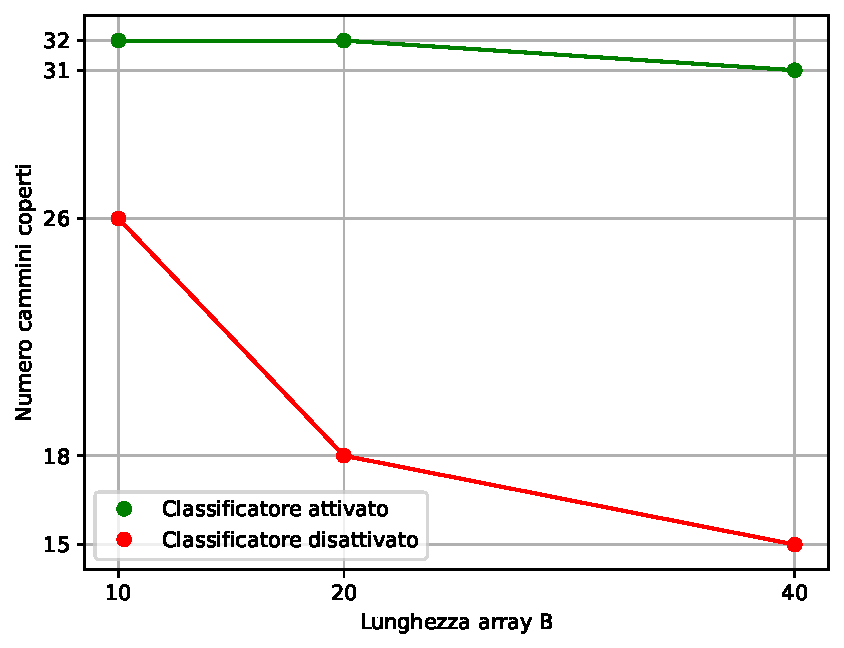
\includegraphics[width=\textwidth]{img/plot.pdf}
  \caption{Grafico con i risultati per MIPC}
  \label{diagram:plot-mipc}
\end{figure}


% --- capitolo 4 - ESPERIMENTI --- %
\chapter{Esperimenti}\label{chapter:experiments}

Questo capitolo ha lo scopo di trattare gli ulteriori esperimenti effettuati dopo l'analisi dei risultati trattata nella sezione \ref{section:results-mipc} per l'esempio MIPC.
\\ \\ Prima di parlare dei nuovi esperimenti, è bene fornire una panoramica riguardo agli strumenti utilizzati.

\section{Strumenti utilizzati}
Innanzitutto, la macchina utilizzata per i nuovi esperimenti è la stessa macchina utilizzata per l'esempio \ref{example:mipc}, dunque le specifiche tecniche si possono trovare nella sezione \ref{section:results-mipc}.
\\ \\ La novità principale consiste nell'utilizzo di \textbf{JaCoCo}.
\\ \\ JaCoCo (Java Code Coverage) \cite{bilal2021jacoco} è una libreria gratuita per la copertura del codice in un contesto Java: esegue casi di test JUnit e fornisce un report sulla copertura ottenuta, nel formato desiderato (HTML, XML, CSV, o JSON). \\ \\ Permette di misurare la copertura delle istruzioni e la copertura dei branch di ogni classe e metodo tramite il processo di \qq{bytecode instrumentation}: JaCoCo modifica il bytecode per tenere traccia delle righe di codice coperte durante l'esecuzione dei casi di test. \\ \\ La copertura, sia delle istruzioni sia dei branch, viene calcolata anche sui metodi privati (e sui metodi delle classi innestate), quindi i valori percentuali presenti nel report di JaCoCo danno un'idea effettiva di quanto codice è stato eseguito senza tener conto della visibilità.
\clearpage \noindent L'invocazione a JaCoCo è l'ultimo step della sequenza di operazioni svolte per eseguire singolarmente un benchmark, in quanto i casi di test generati da TARDIS possono essere passati a JaCoCo solo una volta che TARDIS termina la propria esecuzione. 
\\ \\ In particolare, sono stati scritti degli script \textbf{Bash} per automatizzare tutto il processo, che comprende i seguenti task:
\begin{itemize}[label=$\bullet$, itemsep=0pt, topsep=2pt]
    \item la scelta del benchmark (una specifica classe di un progetto) da considerare e la scelta sull'indice di infeasibility (cioè se attivarlo o disattivarlo)
    \item la ripetizione per 3 volte dei seguenti punti:
    \begin{itemize}[label={--}, itemsep=0pt, topsep=0pt]
        \item l'esecuzione di TARDIS, in cui si ha come target la classe corrispondente al benchmark (questo significa che la tecnica DSE viene applicata generando arbitrariamente un caso di test per ciascuno dei metodi pubblici di quella classe)
        \item l'esecuzione di JaCoCo, in cui vengono passati i casi di test generati da TARDIS, e infine la generazione di un report HTML per l'intera classe considerata
    \end{itemize}
    \item l'organizzazione a livello di directory delle esecuzioni svolte e dei report, per facilitare la distinzione dei dati dei diversi esperimenti ed eliminare file non necessari
\end{itemize}
\noindent \\ Per ogni benchmark e per ogni possibile scelta dell'indice di infeasibility (true o false) si hanno 3 esecuzioni perché, come visto anche nella sezione \ref{section:results-mipc}, EvoSuite può commettere errori e avere più dati a disposizione per ogni specifico benchmark aiuta a comprendere se il numero di casi di test che riesce a generare TARDIS nel budget di tempo prestabilito è veramente limitato ad un numero simile a ciò che si sta osservando, oppure si sta considerando un'esecuzione \qq{sfortunata}. \\ In primo luogo il dato che viene esaminato è il \textbf{numero di test generati} da TARDIS, mentre la \textbf{copertura} calcolata da JaCoCo è un ulteriore dato utilizzato per avere un'altra visione dei risultati in termini di percentuale di codice coperto nelle esecuzioni con il classificatore attivato e nelle esecuzioni che non usano il classificatore. \\ \\ Quindi, per \textbf{ogni benchmark} vi sono \textbf{6 esecuzioni} prese in esame: 3 con l'indice di infeasibility attivato e 3 con l'indice di infeasibility disattivato.
\clearpage \noindent Di seguito viene riportato uno schema che illustra quanto appena discusso, dalla scelta di un benchmark (classe) fino alla generazione di report JaCoCo (in HTML).
\begin{figure}[h]
  \centering
  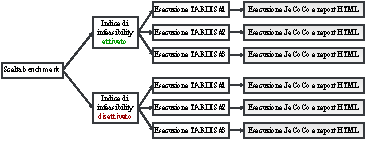
\includegraphics[width=\textwidth]{img/benchmark-diagram.pdf}
  \caption{Task principali svolti in automatico per ogni benchmark con lo scopo di generare report JaCoCo, che contengono la copertura delle istruzioni e dei branch (ossia uno dei due dati considerati durante l'analisi dei risultati, mentre l'altro consiste banalmente in quanti casi di test ha generato TARDIS)}
  \label{diagram:benchmark}
\end{figure}

\section{Parametri e benchmark utilizzati}
In questa sezione vengono trattati i parametri di configurazione utilizzati durante gli esperimenti e brevemente in cosa consistono i benchmark.
\\ \\ Prima di tutto, alcuni parametri di configurazione rimangono invariati rispetto a quelli visti nella sezione \ref{section:results-mipc}, di seguito le \textbf{differenze}:
\begin{itemize}[itemsep=0pt, topsep=2pt]
    \item vengono usati \textbf{5 threads JBSE} al posto di 1
    \item il budget di tempo per ciascun processo di \textbf{EvoSuite} è di \textbf{7.5 minuti}, cioè 450 secondi che sostituiscono il precedente budget di 5 minuti
    \item vi è una nuova limitazione: la \textbf{massima profondità di esplorazione di un caso di test} è impostata a \textbf{50}, ciò significa che dopo aver esaminato 50 branch alternativi si abbandona un caso di test in termini di generazione di path condition alternative
\end{itemize}
\clearpage \noindent In particolare, l'ultimo punto consente di non sprecare il budget di tempo globale per l'esplorazione di pochi casi di test e di abbandonarli ad un certo punto, proseguendo l'esecuzione simbolica dinamica con gli altri casi di test, perciò si ha l'obiettivo di evitare di soffermarsi sulla generazione di troppe path condition alternative con lo stesso caso di test nel momento in cui la path condition è composta da un numero alto di clausole (e quindi vi sono più di 50 branch nel cammino identificato).
\\ \\ In tutto, i parametri di configurazione risultano: 5 threads JBSE, 5 threads EvoSuite, 5 path condition passate ad EvoSuite alla volta, un budget di tempo globale di 60 minuti, un budget di tempo per ciascun processo di EvoSuite pari a 7.5 minuti e la massima profondità di esplorazione di un caso di test settata a 50. 
\\ La quantità di RAM allocata per ogni esecuzione di TARDIS rimane la stessa, quindi 16 GB come nella sezione \ref{section:results-mipc}.
\\ \\ A questo punto si discute riguardo ai benchmark utilizzati. 
\\ \\ Vengono esaminati 10 benchmark che consistono in \textbf{10 classi} appartenenti ai seguenti \textbf{progetti}: \textbf{Dubbo} (framework usato per RPC e microservizi), \textbf{Fastjson} (libreria che converte JSON string in oggetti Java e viceversa), \textbf{Gson} (libreria per serializzare e deserializzare oggetti Java in JSON), \textbf{Guava} (insieme di librerie Google che forniscono funzionalità per diversi scopi, tra cui primitivi, collection, caching, concorrenza, I/O), \textbf{Commons Imaging} (libreria senza dipendenze che permette di leggere e scrivere in diversi formati di immagine), \textbf{la4j} (libreria che fornisce strutture ed algoritmi di Algebra Lineare), \textbf{PDFBox} (libreria per lavorare con documenti PDF) e \textbf{Weka} (insieme di algoritmi di machine learning).
\\ Ad ogni \textbf{benchmark} vi è associato un nome identificativo a cui corrisponde una classe dei progetti appena citati, in dettaglio:
\begin{enumerate}[itemsep=0pt, topsep=2pt]
    \item \verb|DUBBO-3|: classe StringUtils del progetto Dubbo
    \item \verb|FASTJSON-8|: classe JSONReaderScanner del progetto Fastjson
    \item \verb|GSON-2|: classe LinkedHashTreeMap del progetto Gson
    \item \verb|GUAVA-181|: classe SignedBytes del progetto Guava
    \item \verb|GUAVA-224|: classe UnsignedLongs del progetto Guava
    \item \verb|GUAVA-999|: classe MediaType del progetto Guava
    \item \verb|IMAGE-3|: classe BmpImageParser del progetto Commons Imaging
    \item \verb|LA4J-3|: classe CRSMatrix del progetto la4j
    \item \verb|PDFBOX-214|: classe EndstreamOutputStream del progetto PDFBox
    \item \verb|WEKA-983|: classe EditableBayesNet del progetto Weka
\end{enumerate}

\section{Risultati benchmark}
Questa sezione ha lo scopo di riportare ed analizzare i risultati ottenuti dalle diverse esecuzioni dei benchmark elencati precedentemente.
\\ \\ Di seguito si ha una tabella che indica il \textbf{nome del benchmark} e per ogni esecuzione con l'\textbf{indice di infeasibility} attivato/disattivato \textbf{quanti casi di test} sono stati \textbf{generati} da TARDIS, \textbf{quanti} di essi \textbf{non producono eccezioni} quando eseguiti con JUnit, la \textbf{copertura delle istruzioni} e la \textbf{copertura dei branch} della classe corrispondente al benchmark:
\begin{center}
\begin{longtable}{ |>{\centering\arraybackslash}p{2.5cm}|>{\centering\arraybackslash}p{0.945cm}|>{\centering\arraybackslash}p{0.945cm}|>{\centering\arraybackslash}p{1.01cm}|>{\centering\arraybackslash}p{1.15cm}||>{\centering\arraybackslash}p{0.945cm}|>{\centering\arraybackslash}p{0.945cm}|>{\centering\arraybackslash}p{1.01cm}|>{\centering\arraybackslash}p{1.15cm}|   }
\hline
\multicolumn{9}{|c|}{\textsc{Riepilogo esecuzioni benchmark}} \\
\hline
\makecell{Nome \\ benchmark} & \multicolumn{4}{c||}{\makecell{Indice di infeasibility \\ \textbf{attivato}}} & \multicolumn{4}{c|}{\makecell{Indice di infeasibility \\ \textbf{disattivato}}}\\
\cline{2-9} 
 &\# test generati&\# test eseguiti&\% istruz. coperte&\% branch coperti&\# test generati&\# test eseguiti&\% istruz. coperte&\% branch coperti\\
\hline
\endhead

\multicolumn{9}{r}{{Continua nella prossima pagina}} \\
\endfoot

\endlastfoot

\multirow{3}{*}{DUBBO-3} & 27 & 21 & 68\% & 58\% & \cellcolor{gray!15}114 & 102 & 93\% & 92\%\\
                   & 68 & 61 & 90\% & 87\% & 92 & 80 & 85\% & 85\%\\
                   & \cellcolor{gray!15}116 & 111 & 95\% & 93\% & 43 & 40 & 86\% & 80\%\\
\hline
\multirow{3}{*}{\underline{FASTJSON-8}} & \cellcolor{gray!15}101 & 97 & 82\% & 72\% & \cellcolor{gray!15}125 & 121 & 83\% & 76\%\\
                   & 79 & 74 & 83\% & 77\% & 92 & 90 & 82\% & 77\%\\
                   & 72 & 69 & 75\% & 65\% & 89 & 84 & 79\% & 76\%\\
\hline
\multirow{3}{*}{GSON-2} & \cellcolor{gray!15}184 & 177 & 66\% & 54\% & 88 & 83 & 78\% & 62\%\\
                   & 130 & 120 & 67\% & 58\% & \cellcolor{gray!15}162 & 152 & 53\% & 38\%\\
                   & 143 & 137 & 67\% & 55\% & 110 & 107 & 63\% & 50\%\\
\hline
\multirow{3}{*}{GUAVA-181} & 249 & 238 & 98\% & 95\% & \cellcolor{gray!15}300 & 297 & 99\% & 95\%\\
                   & 182 & 174 & 99\% & 95\% & 66 & 64 & 99\% & 95\%\\
                   & \cellcolor{gray!15}437 & 436 & 100\% & 100\% & 139 & 134 & 96\% & 81\%\\
\hline
\multirow{3}{*}{\underline{GUAVA-224}} & 124 & 120 & 89\% & 85\% & 114 & 112 & 94\% & 92\%\\
                   & 161 & 151 & 89\% & 91\% & 133 & 130 & 87\% & 85\%\\
                   & \cellcolor{gray!15}176 & 172 & 88\% & 92\% & \cellcolor{gray!15}228 & 221 & 91\% & 87\%\\
\hline
\multirow{3}{*}{GUAVA-999} & 92 & 89 & 85\% & 63\% & 88 & 85 & 87\% & 59\%\\
                   & 81 & 75 & 83\% & 55\% & \cellcolor{gray!15}105 & 102 & 84\% & 62\%\\
                   & \cellcolor{gray!15}109 & 104 & 83\% & 56\% & 26 & 22 & 79\% & 45\%\\
\hline
\multirow{3}{*}{IMAGE-3} & \cellcolor{gray!15}100 & 95 & 17\% & 11\% & 50 & 40 & 13\% & 9\%\\
                   & 54 & 53 & 13\% & 12\% & 30 & 27 & 10\% & 9\%\\
                   & 55 & 53 & 16\% & 9\% & \cellcolor{gray!15}84 & 81 & 19\% & 14\%\\
\hline
\multirow{3}{*}{\underline{LA4J-3}} & 88 & 83 & 69\% & 59\% & 140 & 131 & 83\% & 77\%\\
                   & \cellcolor{gray!15}107 & 102 & 78\% & 70\% & \cellcolor{gray!15}193 & 184 & 79\% & 66\%\\
                   & 52 & 46 & 58\% & 44\% & 153 & 146 & 82\% & 77\%\\
\hline
\multirow{3}{*}{PDFBOX-214} & 93 & 92 & 97\% & 80\% & \cellcolor{gray!15}87 & 86 & 96\% & 90\%\\
                   & 77 & 76 & 99\% & 95\% & 70 & 70 & 100\% & 97\%\\
                   & \cellcolor{gray!15}97 & 94 & 99\% & 95\% & 86 & 85 & 97\% & 90\%\\
\hline
\multirow{3}{*}{WEKA-983} & 334 & 325 & 30\% & 26\% & \cellcolor{gray!15}388 & 381 & 28\% & 25\%\\
                   & 140 & 119 & 19\% & 16\% & 161 & 154 & 25\% & 24\%\\
                   & \cellcolor{gray!15}829 & 818 & 26\% & 23\% & 368 & 360 & 30\% & 26\%\\
\hline
\end{longtable}
\end{center}
\noindent Nella tabella, la sottolineatura di un benchmark indica che il numero massimo di casi di test generati nelle 3 esecuzioni che non usano il classificatore è maggiore rispetto a quello ottenuto considerando le 3 esecuzioni con il classificatore attivato, mentre le evidenziature di alcune celle mostrano esattamente quali sono i numeri in questione.
\\ \\ Considerando il numero massimo di casi di test generati (si considera questo dato perché ci si aspetta di generare più casi di test evitando le path condition non soddisfacibili) nelle esecuzioni effettuate, si può concludere che in \textbf{7 benchmark su 10} si riscontra un \textbf{miglioramento} con il classificatore.
\\ \\ La copertura, sia delle istruzioni sia dei branch, e il numero di casi di test generati non sono necessariamente correlati, in quanto ad esempio nell'ultimo benchmark (\verb|WEKA-983|) nella terza esecuzione col classificatore si osserva che 829 casi di test portano a una copertura delle istruzioni pari al 26\%, mentre nella prima esecuzione (sempre tra quelle in cui si usa il classificatore) alla generazione di 334 casi di test corrisponde una copertura delle istruzioni del 30\%. \\ Questo è dovuto al fatto che nei casi di test si hanno chiamate indirette a metodi privati e JaCoCo tiene conto di ogni metodo senza considerare la visibilità, così come il fatto che EvoSuite richiama diversi metodi per soddisfare una determinata path condition. Nonostante ciò, considerare anche la copertura può tornare utile per avere un altro punto di vista e sapere se in generale vi è una maggior copertura del codice con l'utilizzo del classificatore. \\ Tornando ad osservare il numero di casi di test generati, per tentare di valutare l'efficacia del classificatore si potrebbero fare delle stime molto approssimative basate sulle esecuzioni migliori:
\begin{itemize}[label=$\bullet$, itemsep=0pt, topsep=2pt]
    \item in \verb|DUBBO-3| si hanno solo 2 casi di test in più
    \item in \verb|FASTJSON-8| si hanno 24 casi di test in meno
    \item in \verb|GSON-2| si hanno 22 casi di test in più
    \item in \verb|GUAVA-181| si hanno ben 137 casi di test in più
    \item in \verb|GUAVA-224| si hanno 52 casi di test in meno
    \item in \verb|GUAVA-999| si hanno solo 4 casi di test in più
    \item in \verb|IMAGE-3| si hanno 16 casi di test in più
    \item in \verb|LA4J-3| si hanno 86 casi di test in meno
    \item in \verb|PDFBOX-214| si hanno 10 casi di test in più
    \item in \verb|WEKA-983| si hanno la bellezza di 441 casi di test in più
\end{itemize}
\noindent \\ Con questi dati a disposizione, si può affermare che il classificatore risulta \textbf{efficace} nella maggior parte degli esperimenti e inoltre i peggioramenti (al massimo 86 test) sono molto più limitati rispetto ai miglioramenti (al massimo \textbf{441} test).
\\ \\ Nella pagina seguente vengono riportati degli istogrammi per visualizzare chiaramente quanto appena trattato.
\clearpage
\begin{figure}[h]
  \centering
  \resizebox{0.7\textwidth}{!}{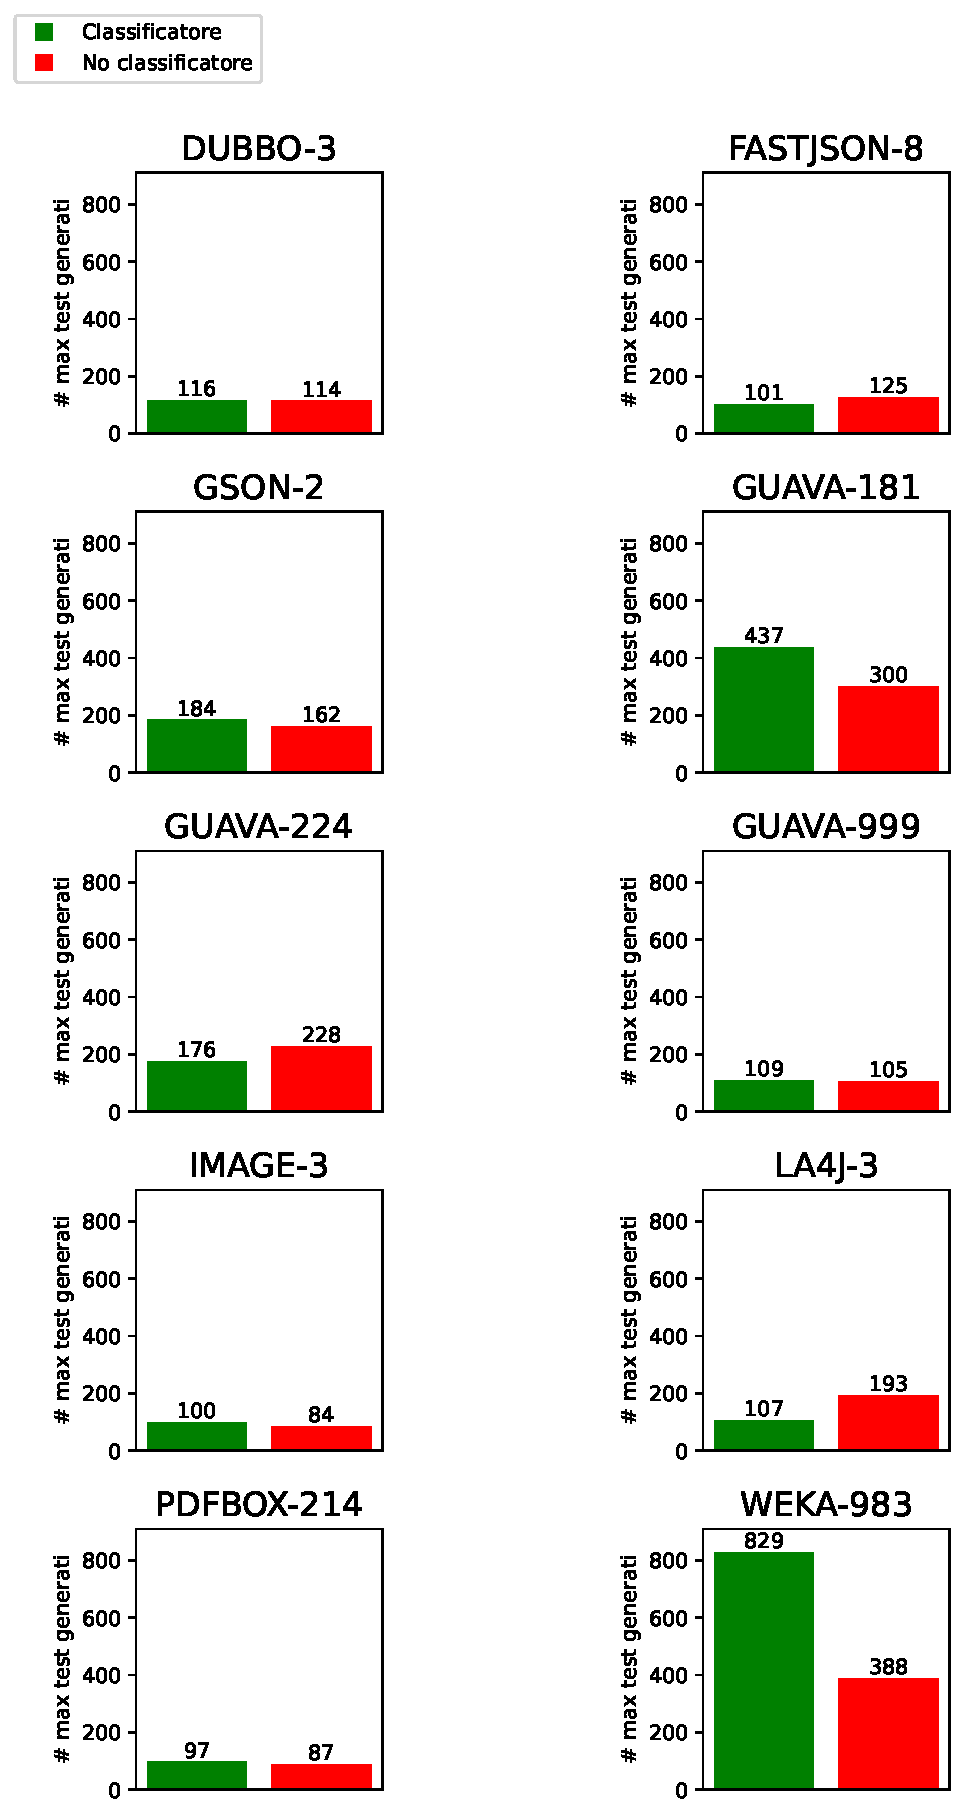
\includegraphics{img/histograms.pdf}}
  \caption{Grafici con i risultati per i benchmark}
  \label{diagram:histograms}
\end{figure}


% --- capitolo 5 - CONCLUSIONI --- %
\chapter{Conclusioni}

In questa trattazione è stato affrontato il problema di migliorare l'efficienza della tecnica DSE avendo a disposizione un budget di tempo limitato, per aumentare il numero di casi di test generati: l'approccio che è stato presentato consente di classificare le nuove path condition alternative e di assegnare priorità diverse.
\\ \\ Dai risultati per l'esempio \ref{example:mipc} (\textbf{MIPC}) è stato possibile dedurre che l'euristica permette di distinguere chiaramente le esecuzioni in cui il classificatore è stato attivato, con \textbf{risultati notevoli}, da quelle in cui esso è stato disattivato: si può affermare che risulta particolarmente efficace per questo esempio.
\\ In seguito sono stati esaminati\textbf{ classi \qq{reali}}, ossia classi appartenenti a progetti attuali di una certa complessità, in cui la tecnica di esecuzione simbolica dinamica è stata applicata a tutti i metodi della classe considerata, aumentando il numero di clausole appartenenti alle condizioni di eseguibilità ottenute dall'esecuzione dei casi di test, in quanto EvoSuite, essendo un generatore di casi di test che utilizza un algoritmo genetico, invoca diversi metodi per soddisfare una determinata path condition (inoltre non si deve dimenticare che EvoSuite non è infallibile, soprattutto quando le path condition sono molto elaborate, e che quando fallisce si ha l'inquinamento del training set, portando a future classificazioni errate). Nonostante le \textbf{difficoltà aggiuntive} dovute all'analisi di programmi reali, dai risultati degli esperimenti si può notare che \textbf{i miglioramenti hanno superato i peggioramenti}, sia in termini di numero di classi in cui si è rilevato un miglioramento rispetto al numero totale di benchmark, sia se si confronta il numero massimo di casi di test generati in più con il numero massimo di casi di test generati in meno.
\\ \\ In futuro si potrebbe provare ad ampliare il numero di benchmark per non basarsi solo su 10 classi, così come si potrebbe provare ad estendere il numero di esecuzioni svolte per ognuno, per avere più dati a disposizione ed effettuare un'analisi più approfondita. \\ Dal punto di vista implementativo, sicuramente sviluppi futuri prevedono il refactoring del codice e la stesura completa della Javadoc (che attualmente per qualche motivo è presente solo parzialmente). Inoltre, nel progetto TARDIS, attualmente è presente una classe (\verb|TreePath|) che implementa una struttura ad albero usata per controllare se una path condition alternativa risulta ridondante o meno: per effettuare il confronto si controlla nodo per nodo, dove ad ogni nodo corrisponde una clausola, e ciò non è particolarmente efficiente sia in termini di spazio sia in termini di tempo (poiché con il proseguire dell'esecuzione si hanno sempre più clausole da gestire). Questo è uno dei motivi per cui TARDIS risulta costoso in termini di risorse (infatti per gli esperimenti sono stati allocati 16 GB di RAM). \\ Quindi, tra le prospettive future non manca l'ottimizzazione dello spazio e del tempo in TARDIS per le classi esistenti, per permettere di includere più efficientemente l'euristica nel progetto ed evitare che path condition con un numero elevato di clausole possano rallentarne il funzionamento e far sprecare tempo prezioso.
\\ \\ Concludendo la trattazione, sono stati raggiunti gli obiettivi prestabiliti per questa esperienza e i risultati sono incoraggianti per sostenere che la strada intrapresa sia quella giusta.

\clearpage

% --- BIBLIOGRAFIA --- %
\printbibliography

\end{document}